\documentclass[12pt]{report}
\usepackage{geometry}
\geometry{letterpaper}
%\usepackage[parfill]{parskip}    % Activate to begin paragraphs with an empty line rather than an indent
\usepackage{graphicx}
\usepackage{amscd}
\usepackage{amsmath}
\usepackage{amssymb}
\usepackage{amsthm}
\usepackage{epstopdf}
\usepackage{xxcolor}
\usepackage[pdftex,colorlinks=true,linkcolor=black,citecolor=black,urlcolor=blue]{hyperref}
%\usepackage[UglyObsolete]{diagrams}
\usepackage{diagrams}
\usepackage{amsfonts}

%\usepackage{hyperref}
%[/sw/share/texmf-dist/tex/latex/diagrams/diagrams.sty]
%\usefile{/sw/share/texmf-dist/diagrams.sty}

\oddsidemargin=18pt
\evensidemargin=18pt

\newcommand{\dd}{{\boldsymbol{d}}}
\newcommand{\ee}{{\boldsymbol{e}}}
\newcommand{\ii}{{\boldsymbol{i}}}
\newcommand{\jj}{{\boldsymbol{j}}}
\newcommand{\DD}{\boldsymbol{D}}

\DeclareMathSymbol{\CC}{\mathalpha}{AMSb}{"43}
\DeclareMathSymbol{\NN}{\mathalpha}{AMSb}{"4E}
\DeclareMathSymbol{\QQ}{\mathalpha}{AMSb}{"51}
\DeclareMathSymbol{\RR}{\mathalpha}{AMSb}{"52}
\DeclareMathSymbol{\ZZ}{\mathalpha}{AMSb}{"5A}

\DeclareMathOperator{\ar}{Arg}
\DeclareMathOperator{\re}{Re}
\DeclareMathOperator{\dxp}{dxp}
\DeclareMathOperator{\srt}{srt}
\DeclareMathOperator{\slog}{slog}
\DeclareMathOperator{\ssqrt}{ssqrt}
\newcommand{\iter}[2]{{#1}^{\circ #2}}


\newcommand{\boxhyper}[3]{{#2}\,\boxed{\!{#1}\!}\,{#3}}
\newcommand{\boxhyperlog}[3]{{}_{#2}^{#1}{\begin{tabular}{|c}$\!\!{#3}\!\!$\\\hline\end{tabular}}}
\newcommand{\boxhyperroot}[3]{{}^{#2}_{#1}{\begin{tabular}{|c}\hline\!\!$#3$\!\!\end{tabular}}}

\newcommand{\tower}{\text{\rm T}}
\newcommand{\towerlarge}{\parbox[c]{12pt}{\Large {\rm T}}}
\newcommand{\towerhuge}[2]{{\:}\overset{#2}{\underset{#1}{\parbox[c]{16pt}{\Huge {\rm T}}}}{\:}}

\newcommand{\pentatower}{\text{\rm \bf 4}}
\newcommand{\pentatowerlarge}{\parbox[c]{9pt}{\Large {\rm \bf 4}}}
\newcommand{\pentatowerhuge}[2]{{\:}\overset{#2}{\underset{#1}{\boxed{\parbox[c]{12pt}{\Large {\rm 4}}}}}{\:}}

\newcommand{\stirfirst}[2]{\genfrac{[}{]}{0pt}{}{#1}{#2}}
\newcommand{\stirsec}[2]{\genfrac{\{}{\}}{0pt}{}{#1}{#2}}

\theoremstyle{plain}
\newtheorem{thm}[equation]{Theorem}
\newtheorem{cor}[equation]{Corollary} 
\newtheorem{lem}[equation]{Lemma}
\newtheorem{prop}[equation]{Proposition}
\newtheorem{conj}[equation]{Conjecture}
\newtheorem{question}[equation]{Question}
\newtheorem{oquestion}[equation]{Open Question}
\newtheorem{series}[equation]{Series}
\theoremstyle{definition} 
\newtheorem{defn}[equation]{Definition} 
\theoremstyle{remark} 
\newtheorem{rem}[equation]{Remark} 
\newtheorem{ex}[equation]{Example} 
\newtheorem{notation}[equation]{Notation} 
\newtheorem{term}[equation]{Terminology}


\begin{document}

\title{\bf \Huge Tetration Reference}
\author{
Henryk Trappman \\
Andrew Robbins
}
\date{
\today
\vskip1cm 
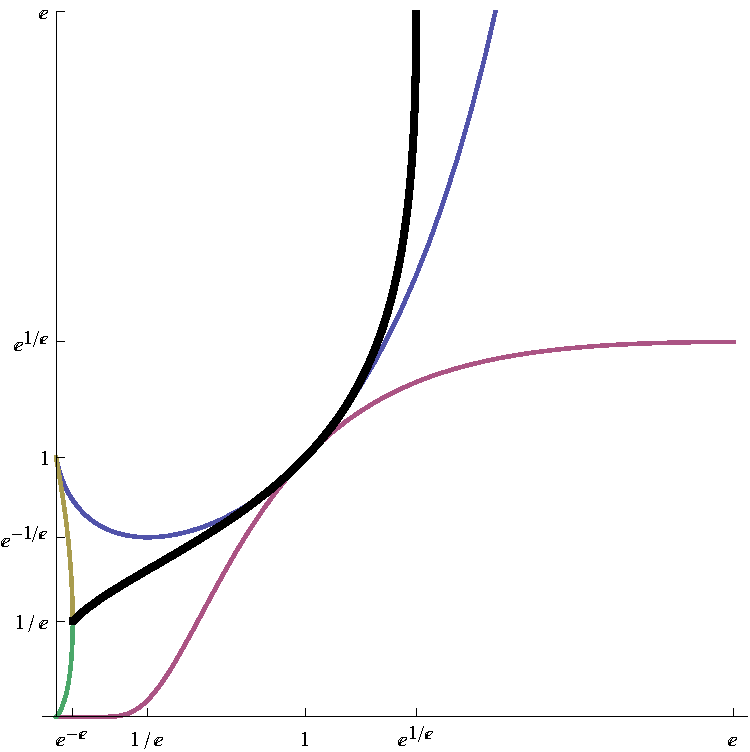
\includegraphics[width=4in]{images/plot-selfroot-plus.pdf} 
}

\maketitle
\pagebreak
\tableofcontents

%########################################
%########################################
%########## Chapter: Introduction
%########################################
%########################################

\chapter{Introduction}
%20070809 Trappmann's 1 "Preamble"
This Reference is meant to provide an in-depth, detailed understanding about tetration and its related topics. 
%The theme enjoys great popularity among pupils and lay mathematicians. One burning 
%question is: What is the most beautiful/suitable/natural extension of tetration to the real 
%numbers? We see already that this question is slightly outside the realm of mathematics 
%more in the realm of taste. Perhaps this is also the reason why professional mathematicians 
%barely considered this question. 

%A more mathematical task would be to find one or more uniqueness conditions for a real extension of tetration. 
%However there are none known yet. And so this Reference also aims to briefly 
%present the various extensions already constructed by various authors in a sense of a fair 
%competition (for appeal to the taste of the reader). [Note however that it will take some 
%time until finished.] 

%The Reference should stop researchers from reinventing the wheel and instead focus their light on undeveloped regions. A special request is to also reveal dead-end ideas, to prevent authors from wasting their efforts there. It is hoped that this Reference makes research about tetration more effective and fruitful. 

The Reference need not be understandable by everyone, and may include advanced topics. 


\section{Classification}

\section{Exponentiation}
%20070809 Trappmann's 3.2 "Extension of the Exponentiation Operation"

{Exponentiation}
Exponentiation is a binary operation on $\CC$ defined by:
\begin{center}
\begin{tabular}{|c|c|c|c|c|}
\hline
$b^1 := b$ &
$b^a := bb^{a-1}$ &
$b^a := \ee^{\ln(b)a}$ &
$\ee^x := \underset{k=0}{\overset{\infty}{\sum}}\frac{x^k}{k!}$ &
$\ln(x) := \underset{k=1}{\overset{\infty}{\sum}}\frac{(1-x)^k}{-k}$ \\
\hline
\end{tabular}
\end{center}

{Table of Values.} Exponentiation near singularities can be summarized by:
\begin{center}
\begin{tabular}{c||c|c|c|c|c|}
&$a = -\infty$&$\Re(a)<0$&$\Re(a)=0$&$\Re(a)>0$&$a=\infty$ \\
\hline
\hline
$b=0$ & $\infty$ & $\infty$ & $\frac{0}{0}$ & 0 & 0 \\
\hline
$0<|b|<1$ & $\infty$ & $b^a$ & $b^a$ & $b^a$ & 0 \\
\hline
$|b|=1$ & $\frac{0}{0}$ & $\ee^{\ii \theta}$ & $\left\{\begin{array}{ll}
1 & \text{if }a = 0, \\
1 & \text{if }b = 1, \\
\ee^{\ii \theta} & \text{otherwise}
\end{array}\right\}$ & $\ee^{\ii \theta}$ & $\frac{0}{0}$ \\
\hline
$|b|>1$ & 0 & $b^a$ & $b^a$ & $b^a$ & $\infty$ \\
\hline
$|b|=\infty$ & 0 & 0 & $\frac{0}{0}$ & $\infty$ & $\infty$ \\
\hline
\end{tabular}
\end{center}
where $\infty$ is complex infinity, and $\frac{0}{0}$ is an indeterminate value. The expression $\ee^{\ii \theta}$ is meant to indicate that the result has magnitude 1, with the angle or argument: $\theta = a\ar(b)$.


%########################################
%########################################
%########## Chapter: Hyper-operations
%########################################
%########################################

\chapter{Hyper-operations}

Hyper-operations are a generalization of the normal sequence of binary operations that are ubiquitous in mathematics and science.
The sequence of binary operations: addition, multiplication, and exponentiation, continues beyond exponentiation \cite{GeislerTO}, but this continuation is not unique. The term {\bf hyper-operation} refers to any binary operation on $\NN$ defined recursively in terms of the operations that come before it. There are quite a few continuations of this sequence, and any set that includes these operations can be called a {hyper-operation} set. It is customary to assign addition to hyper-1 and multiplication to hyper-2, but a different {\bf operation succession} can result in different operations beyond exponentiation. 

The {\bf standard hyper-operations} use
\begin{equation}
\boxhyper{n}{b}{c} = \boxhyper{n-1}{b}{\left(\boxhyper{n}{b}{(c-1)}\right)}
\end{equation}
as the definition of operation succession, and the operations defined from this form what is called {\it the} {\bf hyper-operation sequence}. A common name for this sequence is the Ackermann function, specifically the three argument version. The Ackermann function can either refer to the 2 or 3 argument versions, defined as
\begin{align}
A_2(n, m) & = (\boxhyper{n}{2}{(m+3)}) - 3 \\
A_3(p, n, m) & = \boxhyper{n}{p}{m}
\end{align}
respectively. Since the three argument Ackermann function is identical with the standard hyper-operations, we will use the later for both notation and terminology. Another concept is the more general Grzegorczyk or Grzegorczyk-Wainer hierarchy.

The $n$th hyper-operation is called the {\bf hyper}-$n$-{\bf operation}\footnote{
All of these terms can be generalized from hyper-$N$-{\it{term}} to hyper-{\it{term}} to refer to all ranks.
} or {\bf hyper}-$n$ for short, so hyper-1 is addition, hyper-2 is multiplication, hyper-3 is exponentiation, and so on. In 1947, Robert L. Goodstein \cite{Goodstein1947} coined terms for hyper-operations above hyper-3. His terminology borrows from the Greek number prefixes, so hyper-4 is {\bf tetration}\footnote{Two other terms for tetration are hyper-4 and iterated exponentials. The term {\it $n$th tetrate} is rather new; previous terms were {\it tower}, {\it hyperpower}, and {\it power tower}. The term {\it tetrational} was coined by Holmes as {\it antitetrational}, used in his draft proposal for {\it Composite Arithmetic}.
}, hyper-5 is {\bf pentation}, hyper-6 is {\bf hexation}, and so on.
In general the {\it hyper-} prefix denotes all ranks, and the {\it super-} prefix denotes rank 4.

Here is an overview of the terminology used with common hyper-operations:
\begin{center}
\begin{tabular}{l||llll}
$N$ & 2 & 3 & 4 \\
\hline
\hline
hyper-$N$-operation & multiplication & exponentiation & tetration \\
\hline
hyper-$N$-power & multiple & power & tetrate \\
hyper-$N$-exponential & multiple & exponential & tetrational \\
\hline
hyper-$N$-root & division & root & super-root \\
hyper-$N$-logarithm & division & logarithm & super-logarithm \\
\hline
hyper-$N$-base & factor & base & base \\
hyper-$N$-exponent & factor & exponent & height \\
\hline
hyper-$N$-nest & $n$-ary product & nested exponential & nested tetrational
\end{tabular}
\end{center}

Although hyper-operations in general are only defined over $\mathbb{N} \times \mathbb{N}$, the first three are defined over $\mathbb{C} \times \mathbb{C}$. There are several methods for extending the others' domains to complex numbers, which will be discussed later.
%: one based on Fa\'a di Bruno's formula, and one based on Abel's functional equation. These methods
%If $N \in \ZZ$, then the above right-associative hyper-operation sequence is referred to. 
%However, the case where $N$ is a string of \{L, R\} symbols, refers to the {\it mixed} hyper-operations. 
%and to write some kind of infix operation with a number in it. Munafo uses $b^{(n)}c$, and Rubstov and Romerio use 
%invented by [Knuth], and the other by Robert Munafo, although the latter is sufficiently abstract as to be found in many other authors' work. Although Knuth's notatio	n is more widely used, Munafo's notation more closely maps to the hyper$n$ terminology. Since Munafo's notation starts with addition at $n=1$ it is equivalent to the hyper$n$ terminology, but the equivalent of hyper$n$ in Knuth's notation is the up-arrow with a superscript of $(n-2)$.
%Multiplication is defined in terms of iterated addition, and exponentiation is defined in terms of iterated multiplication. Repeating this produces the {\bf hyper-operation sequence} and the {\bf lower-hyper-operation sequence}:

%########## Chapter: Hyper-operations
%########## Section: Standard notations

\section{Standard notations}

There are two major kinds of notations in common use for hyper-operations, one uses an arrow (${\uparrow}^{n}$) and the other uses a box ($\boxhyper{n}{}{}$). Each notation has at least two variants in common use. The box notation coined by Rubstov and Romerio \cite{RubstovRomerio2003} defines addition as 
$\boxhyper{1}{b}{c} = b + c$. The superscript notation coined by Munafo \cite{MunafoLN} is identical to box notation, defined as $b^{(n)}c = \boxhyper{n}{b}{c}$. The arrow notation coined by Knuth defined the arrow as exponentiation, so is offset from the other notations by two, defined as $b{\uparrow}^{n-2}c = \boxhyper{n}{b}{c}$. The arrow notation coined by Bromer is defined as $b{\uparrow}^{n-3}c = \boxhyper{n}{b}{c}$ being offset by three. Next, we discuss these two versions of arrow notation.

\subsection{Box notations}
Rubstov and Romerio coined box notation, which is similar to Munafo's superscript notation ($b^{(n)}c$) since it assigns the same operations to the same values of $n$. Box notation allows the notation of both hyper-logarithms and hyper-roots as well, an advantage that has motivated the use of box notation in this work.
\begin{equation}\notag
\begin{array}{cc}
a = \boxhyper{n}{b}{c} := \left\{\begin{array}{ll}
b + c & \text{if  } n= 1, \\
b & \text{if } n > 1 \text{ and } c = 1, \\
\boxhyper{n-1}{b}{\left(\boxhyper{n}{b}{(c-1)}\right)} & \text{otherwise}.
\end{array}\right\}
&
\begin{array}{l}
b = \boxhyperroot{n}{c}{a} \\
\\
c = \boxhyperlog{n}{b}{a}
\end{array}
\end{array}
\end{equation}

The box notation for hyper-roots $\left(\boxhyperroot{n}{c}{a}\right)$ resembles a lowercase ``r'' for root, and the box notation for hyper-logarithms $\left(\boxhyperlog{n}{b}{a}\right)$ resembles an uppercase ``L'' for log. These notations provide an excellent  mnemonic for remembering which is which, and helps with learning the new notation as well.

\subsection{Arrow notations}
There are two variants of arrow notation, Knuth's and Bromer's, each of which has some logic behind them.
Knuth's up-arrow notation is defined by:

\begin{equation}\notag
\begin{array}{cc}
a = {b}{{\uparrow}^n}{c} := \left\{\begin{array}{ll}
b^c & \text{if  } n = 1, \\
b & \text{if } n > 1 \text{ and } c = 1, \\
{b}{\uparrow}^{n-1}{\left({b}{\uparrow}^{n}{(c-1)}\right)} & \text{otherwise}.
\end{array}\right\}
\end{array}
\end{equation}
which means $b{\uparrow}c = b^c$ (exponentiation) and $b{\uparrow}{\uparrow}c = {}^{c}b$ (tetration). Knuth's up-arrow notation is the primary notation used for hyper-operations, also used in  \cite{WeissteinCRC2002}.

Bromer's \cite{Bromer1987} arrow notation, also used by M{\"u}ller \cite{MuellerRA}, is more general than Knuth's up-arrow notation. Instead of being restricted to the right-associative iteration of succession $(x+1)$, it allows either right-associative or left-associative iteration of {\it any binary operation}. The Bromer-M{\"u}ller arrow notation is defined as:
\begin{align}
b {\uparrow\!\!{A}} c & := b A (b A \cdots A (b A b)) \text{ with $c$ $b$'s} \\
b{\downarrow\!\!{A}} c & := ((b A b) A \cdots A b) A b \text{ with $c$ $b$'s}
\end{align}
where $b{\uparrow}c = {}^{c}b$ and $b{\downarrow}c = b^{b^{(c-1)}}$ in Bromer's and M{\"u}ller's original usage, whereas $b{\uparrow}c = b{\downarrow}c = b^c$ to simulate Knuth's notation.
Since this allows for two notations for every successive operation, we will use $b{\uparrow}c = b^c$, $b{\uparrow}{\uparrow}c = {}^{c}b$ and $b{\downarrow}{\downarrow}c = b^{b^{(c-1)}}$ as the convention of keeping the last two arrows pointing in the same direction.

\begin{center}
\begin{tabular}{lll|lll}
$N$ & Term & Notation & $N$ & Term & Notation \\
\hline
L & hyper-L & $b{\downarrow}{\downarrow}a = b^{b^{(a-1)}}$ & 
R & tetration & $b{\uparrow}{\uparrow}a = \boxhyper{4}{b}{a} = {}^{a}b$ \\
LR & hyper-LR & $b{\downarrow}{\uparrow}{\uparrow}a$ & 
RR & pentation & $b{\uparrow}{\uparrow}{\uparrow}a = \boxhyper{5}{b}{a} $ \\
LL & hyper-LL & $b{\downarrow}{\downarrow}{\downarrow}a$ & 
RL & hyper-RL & $b{\uparrow}{\downarrow}{\downarrow}a$
\end{tabular}
\end{center}


\subsection{Conway's chain notation}
Conway's chained-arrow notation is one of two generalizations of hyper-operations from a ternary operation to an $n$-ary operation.
It is easy to define this notation in terms of iteration notation $f^{\circ n}(x)$, because it embeds iteration. 
In the following definition $\mathbf{x} = a \rightarrow \cdots \rightarrow z$ stands for a partial Conway chain of any length.
\begin{align}
b \rightarrow c & := b^c \\
\mathbf{x} \rightarrow 1 & := \mathbf{x} \\
\mathbf{x} \rightarrow b \rightarrow c & := C\!A_{(\mathbf{x}; c)}(b) \\
C\!A_{(\mathbf{x}; c+1)}(b) & := C\!A_{(\mathbf{x}; c)}^{\circ b}(1)
\end{align}
as you can see, the second-to-last element plays the role of the iterator.

The 3-element Conway chains are equivalent to hyper-operations:
\begin{equation}
b \rightarrow c \rightarrow n = {b}{\uparrow}^n{c}
\end{equation}
%but are still offset by two from standard hyper-operations.
%where:
%\begin{equation}
%C\!A_{(X, c)}(b) := \begin{cases}
%b^c & \text{if } (\mathbf{x} \rightarrow) \text{ is missing}, \\
%X\text{...} \rightarrow b & \text{if } c = 1, \\
%C\!A_{(\mathbf{x}, c-1)}^b(1) & \text{otherwise}.
%\end{cases}
%\end{equation}
%For two and three parameter cases, Conway chains can be defined more simply as:
%\begin{align}
%b \rightarrow c & = b^c \\
%b \rightarrow c \rightarrow n & = \boxhyper{n+2}{b}{c}
%\end{align}

\subsection{Bowers' array notation}

Jonathan Bowers' array notations use arrays to store small positive integers that evaluate to a single number. In Bowers' description \cite{BowersAN} of his array notations, he makes little distinction between an {\it array} and the {\it evaluation} of that array. To make this distinction more clear, parentheses $(\mathbf{a})$ will be used for the array itself, and square brackets $[\mathbf{a}]$ will be used for evaluation. 
%, even though Bowers himself used braces $\{\mathbf{a}\}$ on his website and angle brackets $\langle \mathbf{a} \rangle$ in his images. It seems as though he intended angle brackets to be used for his notation, but since angle brackets are used in XML and HTML, he felt it was easier to use braces. 
Also used is the convention:
$\mathbf{a} = \{a_k\}_{k=1}^{n}$,
meaning $\mathbf{a}$ is a sequence with $n$ elements where the $k$th element is written $a_k$.
In his original description of his array notation, he gives five rules.
Due to the complexity of rules 4 and 5, they have been broken down as follows. 
%: rule 1 covers evaluating length-1 and length-2 arrays, rule 2 covers evaluating arrays ending in 1, rule 3 covers arrays whose second element is 1, rule 5 effects some replacements that are equivalent to the replacements used in the definition of the hyper-operation sequence, and rule 4 covers arrays whose third element is 1 and effects some replacements that are an extension of the hyper-operation sequence to higher indices of the array. 

Let $rule4(\mathbf{a})$ be $\mathbf{a}$ with the following replacements:
\begin{center}
\begin{tabular}{llll}
$a_k$ & $\rightarrow$ & $a_1\text{ for }2 \le k \le (j-2)$ \\
$a_{j-1}$ & $\rightarrow$ & $[\mathbf{a}\vert_{a_2 \rightarrow (a_2-1)}]$ \\
$a_{j}$ & $\rightarrow$ & $a_{j}-1$
\end{tabular}
\end{center}
where $a_i= 1$ for $3 \le i \le (j-1)$ and $a_j \ne 1$, (i.e., $a_j$ is the first non-1 after $a_3$).

Let $rule5(\mathbf{a})$ be $\mathbf{a}$ with the following replacements:
\begin{center}
\begin{tabular}{llll}
$a_2$ & $\rightarrow$ & $[\mathbf{a}\vert_{a_2 \rightarrow (a_2-1)}]$ \\
$a_3$ & $\rightarrow$ & $a_3-1$
\end{tabular}
\end{center}

Using $rule4(\mathbf{a})$, $rule5(\mathbf{a})$, and the array $\mathbf{a} = \{a_k\}_{k=1}^{n} = (a_1\text{, }a_2\text{, }...\text{, }a_n)$:
\begin{equation}
[\mathbf{a}] = \begin{cases}
a_1 & \text{if } n=1, \\
{a_1} + {a_2} & \text{if } n=2, \\
[\{a_k\}_{k=1}^{n-1}] & \text{if } a_n=1, \\
a_1 & \text{if } a_2=1, \\
[rule4(\mathbf{a})] & \text{if } a_3=1, \\
[rule5(\mathbf{a})] & \text{otherwise}.
\end{cases}
\end{equation}
is the evaluation of Bowers' original array notation.

The way this notation is defined, it is equivalent to the hyper-operation sequence for arrays of three elements. Using $\mathbf{a} = (x, y, n)$, the following relationship holds:
\begin{equation}
[b\text{, }c\text{, }n] = \boxhyper{n}{b}{c}
\end{equation}

In Bowers' description, he mentions that Chris Bird proved that 4-element Bowers arrays are ``comparible'' to 4-element Conway chains, but what this means is unclear.

\subsection{Steinhaus-Moser notation}
Hugo Steinhaus coined a notation for large numbers that defined three elements: $n$ inside a triangle means $n^n$, $n$ inside a square means $n$ inside $n$ nested triangles, and $n$ inside a circle means $n$ inside $n$ nested squares. Steinhaus's notation is also called {\bf circle notation}, due to the fact that it uses a circle for nested squares. Leo Moser then extended this notation by defining $n$ inside a $p$-gon ($p$ sided polygon) to mean $n$ inside $n$ nested $(p-1)$-gons. Moser's extension of Steinhaus's notation has been called {\bf polygon notation}. The two forms that are common to both notations are the triangle ($S\!M_3$) and the square ($S\!M_4$), which are defined by:
\begin{align}
S\!M_3(n) & := n^n \\
S\!M_p(n) & := S\!M_{p-1}^{\circ n}(n)
\end{align}
where $S\!M_{p}^{\circ m}(n)$ represents an $n$ inside $m$ nested $p$-gons. 
%An equivalent definition uses the notation $M(n, m, p) = S\!M_p^{[m]}(n)$

Three very popular large numbers that are defined using this notation are:
\begin{itemize}
\item {\bf mega} $:= S\!M_5(2)$
\item {\bf megiston} $:= S\!M_5(10)$
\item {\bf Moser's number} $:= S\!M_{S\!M_5(2)}(2)$
\end{itemize}

%########## Chapter: Hyper-operations
%########## Section: Standard definitions

\section{Standard definitions}

Having the ability to calculate hyper-operations is not sufficient for manipulating expressions involving them. In order to do algebraic manipulations, we also need their inverse functions, and the ability to calculate them as well. All hyper-operations have two inverses, {\bf hyper-roots} and {\bf hyper-logarithms}. For rank 3, roots are ``easier'' to find than logarithms, as they can be defined as $\sqrt[c]{a} = a^{1/c}$, but for all ranks 4 and above, hyper-logarithms seem to be ``easier'' to find than hyper-roots.

\subsection{Hyper-exponentials}
A {\bf hyper-exponential} is a univariate function defined as $f(x) = \boxhyper{n}{b}{x}$. In order to discuss hyper-exponential functions, it is good idea to extend them to continuous or differentiable functions defined on the real or complex numbers. Although no such an extension has been found, there is a generally accepted framework for discussing such extensions. There are two views of this framework:
\begin{description}
\item[Section-based] A hyper-exponential is defined as a collection (a sheaf) of series expansions (sections) that all satisfy the operation succession.
\item[Piece-based] A hyper-exponential is piecewise-defined by the operation succession and is differentiable across the boundary of its {critical piece}.
\end{description}
and the results from both approaches are equivalent. So it makes little difference which approach is taken, since they can both produce differentiable extensions.

Given two {\bf critical piece} functions defined over intervals of length one:
\begin{itemize}
\item $HC_{(b, d)}(c)$ defined over $0 \le b \in \RR$, $c_0 < c < (c_1 = c_0 + 1)$, $d_1 < d \in \RR$, and 
\item $HD_{(b, d)}(c)$ defined over $0 \le b \in \RR$, $c \in \RR$, $d_0 < d < (d_1 = d_0 + 1)$,
\end{itemize}
the standard hyper-operations may be extended to a ternary operation on $\RR$ as:

\begin{equation}\notag
\boxhyper{d}{b}{c} = \begin{cases}
\boxhyper{d+1}{b}{\left(\boxhyperlog{d+1}{b}{c} + 1\right)} & \text{if }  0 \le d < d_0 \\
HD_{(b, d)}(c) & \text{if } d_0 \le d \le d_1 \\
	{\left\{\begin{array}{ll}
	\boxhyperlog{d-1}{b}{\boxhyper{d}{b}{(c+1)}}	& \text{if } c < c_0 \\
	HC_{(b, d)}(c) 							& \text{if } c_0 \le c \le c_1 \\
	\boxhyper{d-1}{b}{(\boxhyper{d}{b}{(c-1)})}	& \text{if } c > c_1
	\end{array}\right\}} & \text{if } d > d_1
\end{cases}
\end{equation}
where the functions that best define $HC_{(b, d)}(c)$ and $HD_{(b, d)}(c)$ remain unknown. This definition effectively pushes all values within the domains of the critical pieces, thus reducing the domain of interpolation. 

\subsection{Hyper-logarithms}

A {\bf hyper-logarithm} is the inverse function of a hyper-exponential.
The extension of hyper-exponentials to $\RR$ requires the extension of hyper-logarithms to $\RR$ as well.

Given the inverse functions of the {\bf critical piece} functions above:
\begin{equation}\notag
\boxhyperlog{d}{b}{a} = \begin{cases}
\boxhyper{d+1}{b}{\left(\boxhyperlog{d+1}{b}{a} - 1\right)} & \text{if } 0 \le d < d_0 \\
HD^{-1}_{(b, d)}(a) & \text{if } d_0 \le d \le d_1 \\
	{\left\{\begin{array}{ll}
	\left(\boxhyperlog{d}{b}{\boxhyper{d-1}{b}{a}}\right) - 1		& \text{if } a < (\boxhyper{d}{b}{c_0}) \\
	HC^{-1}_{(b, d)}(a) 									& \text{if } (\boxhyper{d}{b}{c_0}) \le a \le (\boxhyper{d}{b}{c_1}) \\
	\left(\boxhyperlog{d}{b}{\boxhyperlog{d-1}{b}{a}}\right) + 1	& \text{if } a > (\boxhyper{d}{b}{c_1})
	\end{array}\right\}} & \text{if } d > d_1
\end{cases}
\end{equation}
which completes the framework for extension of hyper-operations to real numbers.

Here is an example of an extension for $c_0=0$ and $d_0=2$:
\begin{align}
HC_{(b, d)}(c) & \approx b^c \\
HD_{(b, d)}(c) & \approx bc \cos^2\left(\frac{d\pi}{2}\right) + b^c \sin^2\left(\frac{d\pi}{2}\right)
\end{align}
where the square indicates a power, not an iterate.

\subsection{Hyper-powers}
A {\bf hyper-power} is a univariate function defined as $f(x) = \boxhyper{n}{x}{c}$.

%TODO
One property that is true of all\footnote{} hyper-power functions is $\boxhyper{n}{x}{2} = \boxhyper{n+1}{x}{x}$

\subsection{Hyper-roots}
A {\bf hyper-root} is the inverse function of a hyper-power.

%TODO

%########## Chapter: Hyper-operations
%########## Section: Other hyper-operations

\section{Other hyper-operations}
%20070809 Trappmann's 6 "Adaption of the Problem"
%20070809 Trappmann's 6.2 "Alternative Bracketings"

All this time we have been talking about the standard {\it right-associative} hyper-operations. If we instead look at {\it left-associative} or even balanced iteration for the definition of operation succession, then we get different sets of hyper-operations.

\subsection{Munafo's lower hyper-operations}
\begin{equation}
b_{(n)} c := (b_{(n)} (c-1))_{(n-1)} c
\end{equation}

TODO 

\subsection{Bromer's mixed hyper-operations}

TODO

\subsection{Frappier's balanced hyper-operations}
\begin{equation}
H\!F_{n}(b, c) := (x \mapsto H\!F_{n-1}(x, x))^{\circ \log_2(c)}(b)
\end{equation}

TODO

\subsection{Robbins' exponential hyper-operations}
\begin{equation}
H\!R_{n}(b, c) = \exp_{\ee} H\!R_{n-1}(\log_{\ee}(b), \exp_{\ee}^{\circ n-3}(c))
\end{equation}

TODO

\subsection{Trappmann's commutative hyper-operations}
%20070809 Trappmann's 6.1 "Making the Exponentiation Associative and Commutative"
\begin{equation}
HT_{n}(b, c) = \exp_{\ee} HT_{n-1}(\log_{\ee}(b), \log_{\ee}(c))
\end{equation}

TODO

\subsection{Trappmann's binary tree arithmetic}
%20070809 Trappmann's 6.3 "Choose a number system that reflects non-associativity"

TODO

%########################################
%########################################
%########## Chapter: Iteration theory
%########################################
%########################################

\chapter{Iteration theory}

Here is an overview of some of the functions we will discuss.
\begin{equation}\notag
\begin{array}{|c|c||c|c|c|}
\hline
f(x) & \iter{f}{t}(x) &\mathcal{A}[f]\text{ (Abel)} & \mathcal{S}[f]\text{ (Schr{\"o}der)} & \mathcal{J}[f]\text{ (Julia)} \\
\hline
z+x & zt + x & x/z & a^{x/z} & z \\
z + ax & z\frac{a^t-1}{a-1} + a^tx & \log_a\left(\frac{z}{a-1} + x\right) & \frac{z}{a-1} + x & \left(\frac{z}{a-1} + x\right)\ln(a) \\
ax & a^tx & \log_a(x) & x & x\ln(a) \\
x^y & x^{y^t} & \log_y(\ln(x)) & \ln(x) & x \ln(x) \ln(y) \\
y^x & \iter{\exp}{t}_{y}(x) & \slog_{y}(x) & y^{\slog_{y}(x)} & ? \\
y^x-1 & \iter{\dxp}{t}_{y}(x) & ? & ? & \ln(\ln(y))? \\
\hline
\end{array}
\end{equation}



%########## Chapter: Iteration theory
%########## Section: Dynamical systems

\section{Dynamical systems}
\subsection{Fixed points}

Just as Taylor series of $f(x)$ can be described around any point with powers of the form $(x - x_0)^n$ we can just as well as describe the same series of $f(x + x_0)$ with powers of the form $x^n$ without any loss of information. The same is true of fixed points. If $x_0 = f(x_0)$ is a fixed point of $f$, then we can always form a new function that behaves similar under iteration, such as $g(x) = f(x + x_0) - x_0$. Iterating this new function gives $\iter{g}{n}(x) = \iter{f}{n}(x + x_0) - x_0$, in which there is no loss of information.

There are two major conventions for denoting the coefficients of a power series. One is the subscript form, and the other is the alphabetic form:
\begin{align}\label{stdPowerSeries}
f(x)
&= f_0 + f_1 x + f_2 x^2 + f_3 x^3 + \cdots \\
&= z + a x + b x^2 + c x^3 + d x^4 + \cdots
\end{align}
and one common thread to both conventions is that they both take the factorials into account. So the relationship between the subscript form and derivatives is 
$n! f_n = \left[\frac{\partial^n f}{\partial x^n}\right]_{x=0}$, and the relationship to convert this to the alphabetic form is to replace $f_n$ with the $n$-th letter of the Roman alphabet.


\subsection{Lyapunov number}

%########## Chapter: Iteration theory
%########## Section: Functional equations

\section{Functional equations}





\subsection{Abel functions}
%20070809 Trappmann's 4.1 "Translation Equation and Abel Equation"
The {\bf principal Abel function} of $f$ is defined as:
\begin{equation}
\mathcal{A}[f](x) := \lim_{n\to\infty}\left(\log_a \iter{f}{n}(x) - n\right)
\end{equation}
where the limit exists, and $a = f'(0)$ as indicated previously. Note that the limit cannot be distributed across the subtraction, since $\lim_{n\to\infty} n = \infty$ which does not converge, so the separate limits do not exist. In many cases, however, the combined limit does exist, and when it does it can be used to solve the functional equation:
\begin{equation}
\mathcal{A}[f](f(x)) = \mathcal{A}[f](x) + 1
\end{equation}
of which any solution can be called an Abel function of $f$. To see how this works for iterated multiples (exponentiation), if $f(x) = ax$, then $\iter{f}{n}(x) = xa^n$, so:
\begin{align}
\mathcal{A}[f](x) 
& = \lim_{n\to\infty}\left(\log_a (xa^n) - n\right) \\
& = \lim_{n\to\infty}\left(\log_a (x) + n - n\right) \\
& = \lim_{n\to\infty}\left(\log_a (x)\right) \\
& = \log_a (x)
\end{align}
which satisfies the functional equation: $\log_a (ax) = \log_a (x) + 1$.

The derivative of the Abel function of $f$ can be expressed as:
\begin{equation}
\frac{\partial}{\partial x}\mathcal{A}[f](x) = \frac{1}{\mathcal{J}[f](x)}
\end{equation}
so, in terms of the Julia function of $f$, the Abel function of $f$ is:
\begin{equation}
\mathcal{A}[f](x) = \int_{x_0}^{x} \frac{dt}{\mathcal{J}[f](t)}
\end{equation}
where $x_0$ is some chosen constant.



\subsection{Schr{\"o}der function}
The {\bf principal Schr{\"o}der function} of $f$ is defined as:
\begin{equation}
\mathcal{S}[f](x) := \lim_{n\to\infty} \left(\frac{\iter{f}{n}(x)}{a^n}\right)
\end{equation}
where the limit exists, and $a = f'(0)$. This is related to the Abel function of $f$ by:
\begin{equation}
\mathcal{S}[f](x) := a^{\mathcal{A}[f](x)}
\end{equation}

\subsection{B{\"o}ttcher function}
\begin{equation}
\mathcal{B}[f](x) := a^{\mathcal{S}[f](x)}
\end{equation}

\subsection{Julia function}
The {\bf principal Julia function} is defined as:
\begin{equation}
\mathcal{J}[f](x) := \left[\frac{\partial}{\partial t}\iter{f}{t}(x)\right]_{t=0}
\end{equation}
which can be shown to be related the the Abel function of $f$ by:
\begin{equation}
\mathcal{J}[f](x) = \frac{1}{\frac{\partial}{\partial x}\mathcal{A}[f](x)}
\end{equation}
where the Abel function of $f$ is non-constant.

but there is more

\begin{equation}
\mathcal{J}[f](\iter{f}{t}(x)) = f'(x) \mathcal{J}[f](x)
\end{equation}
\begin{equation}
\mathcal{J}[\iter{f}{t}](x) = t \mathcal{J}[f](x)
\end{equation}


\begin{oquestion}
The Julia function of $\dxp_b(x) = b^x-1$ is of the form
\begin{equation}
\mathcal{J}_x[{\ee^{ax} - 1}](x)
= \ln(a)\sum_{k=0}^{\infty} \frac{x^k\sum_{i=0}^{\binom{k-2}{2}}C_{ik}a^i}{\prod_{j=1}^{k-1} (a^j - 1)}
\end{equation}
but so far there is no proof, and we do not know the $C_{ik}$. What are the $C_{ik}$?
\end{oquestion}



%########## Chapter: Iteration theory
%########## Section: Special matrices

\section{Special matrices}

The special matrices in this section are all related to power series expansions of functions, so we will start with how to analyze (break apart) a function into matrices, and to synthesize (put together) these matrices back into a function. Starting with the standard notation for power series (\ref{stdPowerSeries}) we can write a function as:
\begin{equation}
f(x) = \sum_{k=0}^{\infty}f_k x^k = \mathbf{F}[f]^T\mathbf{V}(x) = 
\left[\begin{array}{cccc}
f_0 & f_1 & f_2 & \cdots
\end{array}\right]
\left[\begin{array}{c}
1 \\ x \\ x^2 \\ \vdots
\end{array}\right]
\end{equation}
where $\mathbf{F}[f]^T$ is the coefficients of $f$, and $\mathbf{V}(x)$ is a Vandermonde vector of $x$.

% from Gottfried's ContinuousFunctionalIteration.pdf:
There is an important distinction between two types of such powerseries, $f_0=0$ and $f_0\ne0$. These series behave in regard of iteration much differently. Iterations of $f$, where the value of the function is reintroduced as an argument, as in $f(x)$, $f(f(x))$, $f(f(f(x)))$, can be denoted by $\iter{f}{n}(x)$. This discussion considers $f$ as a formal power series, so considerations of convergence can be safely ignored.

To compute the iterates of $f(x)$, we can look first to its second iterate:
\begin{align}
\iter{f}{2}(x) = 
\end{align}

\subsection{Carleman matrix}
Using the vectors we defined above, we can define the Carleman matrix of $f$ as:
\begin{equation}
\mathbf{M}[f] = \left[\begin{array}{c}
\mathbf{F}[1]^T \\ \mathbf{F}[f]^T \\ \mathbf{F}[f^2]^T \\ \vdots
\end{array}\right]
\end{equation}
in which each row is a vector of the coefficients of the $j$-th power of $f$ (not iterate).
We can also reference the elements individually to define it as:
\begin{equation}
\mathbf{M}[f]_{jk} = \frac{1}{k!} \left[\frac{\partial^k}{\partial x^k} (f(x))^j \right]_{x=0}
\end{equation}
which satisfies the functional equation:
\begin{equation}
(f(x))^j = \sum_{k=0}^{\infty} \mathbf{M}[f]_{jk} x^k
\end{equation}
Going back to the vector-based definition of the Carleman matrix, we can see that:
\begin{equation}
\mathbf{M}[f] \mathbf{V}(x)
 = \left[\begin{array}{c}
\mathbf{F}[1] \cdot \mathbf{V}(x) \\ \mathbf{F}[f] \cdot \mathbf{V}(x) \\ \mathbf{F}[f^2] \cdot \mathbf{V}(x) \\ \vdots
\end{array}\right]
 = \left[\begin{array}{c}
1 \\ f(x) \\ f(x)^2 \\ \vdots
\end{array}\right]
= \mathbf{V}(f(x))
\end{equation}
which implies the fundamental property of Carleman matrices: converting function iteration into matrix multiplication. By replacing $f(x) \to \iter{f}{n}(x)$, we get:
\begin{align}
\mathbf{V}(\iter{f}{n}(x)) 
= \mathbf{M}[\iter{f}{n}] \mathbf{V}(x)
\end{align}
and by replacing $x \to \iter{f}{n-1}(x)$ and reducing, we get:
\begin{align}
\mathbf{V}(\iter{f}{n}(x)) 
& = \mathbf{M}[f] \mathbf{V}(\iter{f}{n-1}(x)) \\
& = \mathbf{M}[f]^2 \mathbf{V}(\iter{f}{n-2}(x)) \\
& = \mathbf{M}[f]^n \mathbf{V}(x)
\end{align}
which proves the fundamental property:
\begin{equation}
\mathbf{M}[\iter{f}{n}]
= \mathbf{M}[f]^n
\end{equation}

There are two cases when the Carleman matrix is triangular: linear functions:
\begin{equation}
\mathbf{M}_x[z + ax]
= \left[\begin{array}{cccccc}
1&0&0&0&0&\cdots\\
z&a&0&0&0&\cdots\\
z^2&2za&a^2&0&0&\cdots\\
z^3&3z^2a&3za^2&a^3&0&\cdots\\
z^4&4z^3a&6z^2a^2&4za^3&a^4&\cdots\\
\vdots&\vdots&\vdots&\vdots&\vdots&\ddots
\end{array}\right]
\end{equation}
and functions such as $f(x) = \sum_{k=1}^{\infty}f_kx^k$ where $z=0$ is a fixed point:
\begin{equation}
\mathbf{M}[f]
= \left[\begin{array}{cccccc}
1&0&0&0&0&\cdots\\
0&a&b&c&d&\cdots\\
0&0&a^2&2ab&2ac+b^2&\cdots\\
0&0&0&a^3&3a^2b&\cdots\\
0&0&0&0&a^4&\cdots\\
\vdots&\vdots&\vdots&\vdots&\vdots&\ddots
\end{array}\right]
\end{equation}



\subsection{Bell matrix}
\begin{equation}
\mathbf{B}[f] = \mathbf{M}[f]^T
\end{equation}
So
\begin{equation}
\mathbf{B}[f] = \left[\begin{array}{cccc}
\mathbf{F}[1] & \mathbf{F}[f] & \mathbf{F}[f^2] & \cdots
\end{array}\right]
\end{equation}
We can also reference the elements individually to define it as:
\begin{equation}
\mathbf{B}[f]_{jk} = \frac{1}{j!} \left[\frac{\partial^j}{\partial x^j} (f(x))^k \right]_{x=0}
\end{equation}

\subsection{Abel matrix}
Let
\begin{equation}\notag
\mathbf{1} = 
\left[\begin{array}{c}
1\\0\\0\\\vdots
\end{array}\right]
\quad
\mathbf{J} = 
\left[\begin{array}{cccccc}
1&0&\cdots&0&0\\
0&1&\cdots&0&0\\
\vdots&\vdots&\ddots&\vdots&\vdots\\
0&0&\cdots&1&0
\end{array}\right]
\quad
\mathbf{K} = 
\left[\begin{array}{cccccc}
0&0&\cdots&0\\
1&0&\cdots&0\\
0&1&\cdots&0\\
\vdots&\vdots&\ddots&\vdots\\
0&0&\cdots&1
\end{array}\right]
\end{equation}

The {\bf Abel matrix} of $f$ (of size $n$) is defined as
\begin{equation}
\mathbf{A}[f] := 
\mathbf{J}
(\mathbf{B}[f] - \mathbf{I})
\mathbf{K}
\end{equation}
This can be visualized as the upper-right submatrix of the Bell matrix of $f$, that is the matrix that includes all elements except the first column and the last row.

The power of the Abel matrix is that it encodes the Abel functional equation, or in other words, if 
$\mathbf{A}[f]\mathbf{F}[\alpha] = \mathbf{1}$, then $\mathcal{A}[f](x) = \alpha(x) = (\mathbf{F}[\alpha]\cdot\mathbf{V}(x)) x + C$, where the extra $x$ has been added because the coefficient $\alpha_1$ is now the first element of $\mathbf{F}[\alpha]$ and $C$ is any constant. 
To illustrate with $f(x) = z + ax + bx^2 + \cdots$:
\begin{equation}
\mathbf{A}[f]\mathbf{F}[\alpha] = 
\left[\begin{array}{cccccc}
z&z^2&z^3&\cdots\\
a-1&2az&3az^2&\cdots\\
b&a^2+2bz-1&3a^2z + 3bz^2&\cdots\\
\vdots&\vdots&\vdots&\ddots\\
\end{array}\right]
\left[\begin{array}{c}
\alpha_1\\
\alpha_2\\
\alpha_3\\\vdots
\end{array}\right]
\end{equation}
which implies that $\mathbf{F}[\alpha] = \mathbf{A}[f]^{-1}\mathbf{1}$ if the Abel matrix is invertible.


%########## Chapter: Iteration theory
%########## Section: Regular iteration

\section{Regular iteration}

\subsection{General fixed points $(z=0)$}
According to Daniel Geisler [?]:
\begin{align}
\iter{f}{t}(x)
& = a^t x
\notag\\& + \left(b \sum_{k_1=0}^{t-1}a^{2t-k_1-2}\right) \frac{x^2}{2!}
\notag\\& + \left(c \sum_{k_1=0}^{t-1}a^{3t-2k_1-3} + 3b^2 \sum_{k_1=0}^{t-1} \sum_{k_2=0}^{t-k_1-2}a^{3t-2k_1-k_2-5}\right) \frac{x^3}{3!}
\notag\\& + \cdots \notag
\end{align}

\subsection{Non-parabolic fixed points $(z=0, a \ne 1)$}
\begin{align}
\iter{f}{t}(x)
& = a^t x
\notag\\& + \left(b \frac{a^{t-1}(a^t-1)}{(a-1)}\right) x^2
%\notag\\& + \frac{a^{t-2}(a^t-1) (a (-2 b^2  + (a-1) c) + a^t  (2 b^2  + (a-1) a c)}{(a-1)(a^2-1)} x^3
\notag\\& + \left(
c \frac{a^{t-1}(a^{2t}-1)}{(a^2-1)} + 
b^2 \frac{2 a^{t-2}(a^t-a)(a^t-1)}{(a-1)(a^2-1)} \right) x^3
\notag\\& + \left(
d \frac{a^{t-1}(a^{3t}-1)}{(a^3-1)} \right. \notag\\& \quad +
bc \frac{a^{t-2}(a^t-a)(a^t-1)(a^t(5+3a)+5a+2)}{(a^2-1)(a^3-1)} \notag\\& \quad + \left.
b^3 \frac{a^{t-3}(a^t-a)(a^t-1)(a^t(5+a) -5a^2 -1)}{(a-1)(a^2-1)(a^3-1)} \right) x^4
\notag\\& + \cdots \notag
\end{align}

\subsection{Parabolic fixed points $(z=0, a=1)$}
\begin{align}
\iter{f}{t}(x)
& = x
\notag\\& + btx^2
\notag\\& + \left(ct + b^2t(t-1)\right) x^3
\notag\\& + \left(dt + bc\frac{5}{2}t(t-1) + b^3\frac{1}{2} t(t-1)(2t-3)\right) x^4
\notag\\& + \left(
e t + (2bd + c^2)\frac{3}{2}t(t-1) \right. +
b^2 c \frac{1}{6}t(t-1)(26t-37)\notag\\& \quad +  \left. 
b^4 \frac{1}{3}t(t-1)(t-2)(3t-4)
\right) x^5 
\notag\\& + \cdots \notag
\end{align}



%########## Chapter: Iteration theory
%########## Section: Natural iteration

\section{Natural iteration}

Natural iteration is based entirely on the Abel matrix of $f$. After solving the matrix equation $\mathbf{A}[f]\mathbf{F}[\alpha] = \mathbf{1}$, we obtain the Taylor coefficients of $\alpha(x)$, which can be solved for symbolically. Starting with $f(x) = z + ax + bx^2 + \cdots$, we find that the solutions for the first few approximants $(n=1,2,3)$ are as follows:

\begin{align}
\alpha(x)_1 &= \frac{x}{z} \\
\alpha(x)_2 &= \frac{2azx + (1-a)x^2}{z^2(a+1)} \\
\alpha(x)_3 &= \frac{3a(a^2 + 1)z^2x + 3(bz - a^3 + a^2)zx^2 + (-2bz + a^3 - a^2 - a + 1)x^3}{z^3(bz + a^3 + 2a^2 + 2a + 1)}
\end{align}

%\begin{equation}
%\alpha(x)_2 = \frac{2a}{1+a}\alpha(x)_1+\frac{1-a}{1+a}\alpha(x)_1^2
%\end{equation}
%PS. one of the benefits of F(x)/F(1) is the representation of Julia functions as F(1)/F(x)


%########################################
%########################################
%########## Chapter: Tetration
%########################################
%########################################

\chapter{Tetration}

\begin{question}
How is tetration written?
\end{question}
Tetration can be represented in various other notations as:
\begin{equation}\notag
\begin{array}{rlll}
{{x^{x^{\cdot^{\cdot^{x^x}}}}}} 
& = {}^{n}{x} && \text{(Maurer's left-superscript notation)}
\\ & = \boxhyper{4}{x}{n} && \text{(Romerio's box notation)}
\\ & = x {\uparrow}{\uparrow} n && \text{(Knuth's up arrow notation)}
\\ & = (x \rightarrow n \rightarrow 2) && \text{(Conway's chained arrow notation)}
\\ & = \exp_x^n(1) && \text{(iterated exponential notation)}
\\ & = \towerhuge{k=1}{n}x = \tower^{n}x && \text{(nested exponential notation)}
\end{array}
\end{equation}

%########## Chapter: Tetration
%########## Section: Variants of tetration

\section{History of tetration}

The history of tetration starts with Euler, Eissenstein, Goodstein, Maurer, Lambert, and many other people, depending on which aspect of tetration one is considering. Also, various functions related to tetration, such as iterated exponentials and nested exponentials have been developed by different people at different times.


\subsection{Iterated exponentials}

\begin{question}
How are iterated exponentials written?
\end{question}
Iterated exponentials can be represented in various notations as:
\begin{equation}\notag
\begin{array}{rlll}
{{b^{b^{\cdot^{\cdot^{b^x}}}}}} 
& = \exp_b^n(x) && \text{(Euler's mnemonic notation)}
\\ & = (b{\uparrow})^{n}(x) && \text{(Knuth's notation)}
\\ & = {}^{n}(b, x) && \text{(Galidakis' notation)}
\\ & = {}^{n}b^x && \text{(Robbins' notation)}
\\ & = b^{[n]}(x) && \text{(Campagnolo {\it et.al.} notation)}
\\ & = \towerhuge{k=1}{n} (b; x) = \tower^{n}(b; x) && \text{(nested exponential notation)}
\end{array}
\end{equation}


\subsection{Nested exponentials}

\begin{question}
How are nested exponentials written?
\end{question}
Nested exponentials can be represented as:
\begin{equation}\notag
\begin{array}{rlll}
{{a_1^{a_2^{\cdot^{\cdot^{a_{n-1}^{a_n}}}}}}} 
& = \tower(a_1, a_2, \cdots, a_{n-1}, a_n) && \text{(Barrow-Brunson notation)}
\\ & = \towerhuge{k=1}{n-1} (a_k; a_n) && \text{(Barrow-Shell notation)}
\\ & = \towerhuge{k=1}{n} a_k && \text{(Barrow's notation)}
%\\ & = \towerhuge{k=1}{n-j} (a_k; a_{n-j+1}, \cdots, a_n) && \text{(extended Shell notation)}
%\\ & = \tower(a_1, a_2, \cdots; a_n) && \text{(Shell's infinite notation)}
\end{array}
\end{equation}

{Historical notations and terminology}
\begin{itemize}

%1936
\item{D. F. Barrow} uses the notation $E(a_1, a_2, a_3, \cdots, a_n)= \towerlarge_{k=1}^{n} {a_k}$ and the notation $E_{k=1}^{\infty}a_k = \towerlarge_{k=1}^{\infty} {a_k}$ where he coins the term {\it infinite exponentials} along with many others including the $n$th {\it margerin function} for $z \mapsto \towerlarge_{k=1}^{n} ({a_k}; z)$ in \cite{Barrow}.

%1962
\item{D. L. Shell} uses most of Barrow's terms, the notation $E(a; z)= \exp_a^{\infty}(z)$ and the notation $E(a_1, a_2, a_3, \cdots; z)=  \towerlarge_{k=1}^{\infty} ({a_k}; z)$ in \cite{Shell}

%1957
\item{W. J. Thron} uses 
the notation $T_{n}(z) = \towerlarge_{k=1}^{n} (\ee^{a_k}; z)$ in \cite{Thron1957}.

%1986
\item{G. Bachman} uses the notations $E_n = [a_1, a_2, a_3, \cdots, a_n] = \towerlarge_{k=1}^{n} {a_k}$ in \cite{Bachman}.

%1991
\item{X. Dong} uses the notation $E_{\lambda_1, \cdots, \lambda_n}(z) =  \towerlarge_{k=1}^{n} (\ee^{\lambda_k}; z)$ in \cite{Dong}.

%1995
\item{B. W. Brunson} uses the notation $T(a_1, a_2, a_3, \cdots, a_n)=  \towerlarge_{k=1}^{n} {a_k}$ in \cite{Brunson}.

%1999
\item{V. I. Yukalov and S. Gluzman} use $F_n(t, \tau) = a_0 \towerlarge_{k=1}^{n} (\ee^{a_k/a_{k-1}}; \tau)$ in \cite{YukalovGluzman1999}.

%Mar. 2006
\item{S. Sykora} uses the notations
$E_{\pm}^n(x) = \{b_1b_2b_3\cdots\ |\ x\} = \towerlarge_{k=0}^{\infty} (\beta^{2b_k - 1}; x)$ where $b_k \in \{0, 1\}$ and uses the term {\it binary iterated powers} (misnomer) in \cite{Sykora}. Its acronym {\bf bips} sounds nice, though, so it might be used instead.

%Apr. 2006
\item{N. J. A. Sloane} uses the term {\it tower of height} $n$ for $\towerlarge_{k=1}^{n} {a_k}$ in \cite{Sloane7Seq2006}.

\end{itemize}


Using Barrow's terms, Shell, Thron, Dong, Sykora, and Yukalov {\it et.al.} are actually discussing {\it margerin exponential} functions, although they do not say so explicitly. This provides counter examples for the argument that nested exponentials are too rare to deserve a notation. Clearly, this list would indicate otherwise.

Although $E$ is more commonly used than $T$, it is easily mistakable for $\Sigma$, especially when they appear together 
(for example: $\rm E \ \Sigma \ T \ \Pi$), 
where it can be seen that it is much easier to mistake $E$ for $\Sigma$ than it is to mistake $T$ for $\Pi$. It is for this reason that we use $T$ in this Reference instead of $E$.

\subsection{Exponential forests}

There is a problem posted on a wall of the math club at the University of Maryland, by the author Andrew Snowden. He apparently teaches both there and at Princeton, and poses many interesting problems in mathematics. The problem set was simply called {\it Some More Problems}, and contained problems from algebra and number theory to real and complex analysis. The second problem posted seemed interesting, as it related to nested exponentials, so it will be reproduced here:

\begin{quote}
A natural nummber $n$ may be factored as $n = p_1^{a_1} p_2^{a_2} \cdots  p_n^{a_n}$ where the $p_n$ are distinct prime numbers and $a_n$ are natural numbers. Since the $a_n$ are natural numbers, they may be factored in such a manner as well. This process may be continued, building a ``factorization tree'' until all the top numbers are 1. Thus any question that can be asked of trees (i.e. the height of a tree, the number of nodes in a tree, etc.) may be asked of our natural number $n$. This problem is about the height of $n$ which we denote $h(n)$. Define:
\begin{equation}\notag
D_n = \lim_{N \rightarrow \infty} \frac{1}{N} |\{ k \le N \text{ : } h(k) \ge n \}|
\end{equation}
$D_n$ is sort of the density of numbers with height at least $n$. It is obvious that $D_1 = 1$ since all numbers have height at least 1.
\begin{enumerate}
\item Show that
\begin{equation}\notag
\frac{1}{2} < ({}^{n}2) D_n \le 3
\end{equation}
\item Let $a$ be the average height of a natural number (i.e. if you were to pick many numbers at random their height would average out to $a$). Using the previous part and other methods, give bounds on $a$. The best bounds [Andrew Snowden has found] are
\begin{equation}
1.42333 < a < 1.4618
\end{equation}
\end{enumerate}
\end{quote}

Here are some examples of {\it prime factorization trees} as suggested by Snowden:
\begin{equation}\notag
\begin{array}{r|l}
\text{Number} & \text{Factorization} \\ 
\hline
4 & 2^2
\\ 8 & 2^{3}
\\ 9 & 3^{2}
\\ 12 & 2^2 \cdot 3
\\ 16 & 2^{2^{2}}
\\ 48 & 2^{2^{2}} \cdot 3
\\ 64 & 2^{2 \cdot 3} 
\\ 81 & 3^{2^{2}}
\\ 144 & 2^{2^2} \cdot 3^2
\\ 4096 & 2^{2^2 \cdot 3}
\\ 65536 & 2^{2^{2^{2}}}
\\ 531441 & 3^{2^2 \cdot3}
\\ 7625597484987 & 3^{3^3}
\end{array}
\end{equation}


%########## Chapter: Tetration
%########## Section: Standard definitions

\section{Standard definitions}

Most of the standard definitions of tetration define it recursively:
\begin{align}
{}^{1}x & := x \\
{}^{n+1}x & := x^{\left( {}^{n}x \right)}
\end{align}
such that tetration is only defined for natural number $n$. There are extensions of tetration beyond this domain, but each has a specific domain of applicability. For all complex number $x$ within the Shell-Thron region, one can use regular iteration, and for all complex number $x$ with real part greater than 1, one can use natural iteration, but for other bases, no extension has been found.

\subsection{Super-exponentials (tetrationals)}

\begin{defn}
The base-$b$ {\bf tetrational} function is $x \mapsto {}^{x}b$.
\end{defn}

For some bases, no fancy methods are required, for example, base 0 and base 1. For base-0 tetrational functions, 


\subsection{Super-logarithms}
\begin{defn}
The base-$b$ {\bf super-logarithm} is the inverse of the base-$b$ tetrational.
\end{defn}

Using the third interpretation of super-logarithms (i.e. the number of times you must apply a logarithm before one is obtained), we can define integer versions as:
\begin{align}
\lfloor \slog_x(z) \rfloor & = \begin{cases}
-2 & \text{if } z < 0, \\
\lfloor \slog_x(\log_x(z)) \rfloor + 1& \text{if } z \ge 0.
\end{cases}\\
\lceil \slog_x(z) \rceil & = \begin{cases}
-1 & \text{if } z \le 0, \\
\lceil \slog_x(\log_x(z)) \rceil + 1& \text{if } z > 0.
\end{cases}
\end{align}
[superlogarithm base 1]
[superlogarithm base infty]

\subsection{Super-powers (tetrates)}
\begin{defn}
The $n$-th {\bf tetrate} function is $x \mapsto {}^{n}x$.
\end{defn}


\begin{thm}[Galidakis]
For $x \in \CC$ and $0 \le n \in \ZZ$:
\begin{equation}
{}^{n}{x} = \sum^\infty_{k=0} p_{nk} \log(x)^k
\end{equation}
where:
\begin{equation} \label{defP}
p_{nk} = \begin{cases}
1 & \text{if } n \ge 0 \text{ and } k = 0, \\
0 & \text{if } n = 0 \text{ and } k > 0, \\
\frac{1}{k!} & \text{if } n = 1, 
\end{cases}
\end{equation}
otherwise:
\begin{equation}\label{recurP0}
\boxed{
p_{nk} = \frac{1}{k} \sum^k_{j=1} j p_{n(k-j)} p_{(n-1)(j-1)}
}
\end{equation}
and Galidakis gives the recurrence equation (\ref{recurP0})  in [?].
\end{thm}
\begin{thm}[Robbins]
For $x \in \CC$ and $0 \le n \in \ZZ$:
\begin{equation}
{}^{n}{x} = \sum^\infty_{k=0} t_{nk} (x-1)^k
\end{equation}
where:
\begin{equation} \label{defT}
t_{nk} = \begin{cases}
1 & \text{if } n \ge 0 \text{ and } k = 0, \\
0 & \text{if } n = 0 \text{ and } k > 0, \\
1 & \text{if } n = 1 \text{ and } k = 1, \\
0 & \text{if } n = 1 \text{ and } k > 1,
\end{cases}
\end{equation}
otherwise:
\begin{equation}\label{recurT1}
\boxed{
t_{nk} = \frac{1}{k} \sum^k_{j=1} \frac{1}{j} \sum^k_{i=j} i {(-1)^{j-1}} t_{n(k-i)} t_{(n-1)(i-j)}
}
\end{equation}
\end{thm}

\subsection{Super-roots}
\begin{defn}
The $n$-th {\bf super-root} is $\srt_n(z) = x$ if and only if ${}^{n}x = z$.
\end{defn}
A {\it super-root} is an inverse function of tetration, 
or to be more specific, the inverse of a hyperpower function. 


%{Lagrange inverse series}
Before we can go into more detail about series expansions of super-roots, we must first recall the process of finding a power series for an inverse function, given a power series for the function itself. This process is called Lagrange inversion [?] (sometimes confused with Lagrange reversion).
Lagrange inverse series:


\subsection{Iterated exponentials}
\begin{defn}
The $n$-th base-$b$ {\bf iterated exponential} is $\exp_b^n(x)$.
\end{defn}

Generally speaking, there are three variables in a iterated exponential, so there are at least three different ways of forming a power series expansion of them. For series expansions of $\exp_b^{c}(a)$, series about $a = ({}^{\infty}b)$ are usually discussed in {\it regular iteration}, and series about $c=0$ are usually discussed in {\it natural iteration} but series in $b$ are specific to tetration, so these expansions are covered here.

\begin{thm}[Galidakis]
For $x \in \CC$, $z \in \CC$ and $0 \le n \in \ZZ$:
\begin{equation}
{}^{n}(x; z) = \sum^\infty_{k=0} p_{nk}(z) \log(x)^k
\end{equation}
where:
\begin{equation} \label{defPz}
p_{nk}(z) = \begin{cases}
1 & \text{if } n > 0 \text{ and } k = 0, \\
z & \text{if } n = 0 \text{ and } k = 0, \\
0 & \text{if } n = 0 \text{ and } k > 0, \\
\frac{z^k}{k!} & \text{if } n = 1, 
\end{cases}
\end{equation}
otherwise:
\begin{equation}\label{recurP0z}
\boxed{
p_{nk}(z) = \frac{1}{k} \sum^k_{j=1} j p_{n(k-j)}(z) p_{(n-1)(j-1)}(z)
}
\end{equation}
\end{thm}
\begin{thm}[Robbins]
For $x \in \CC$, $z \in \CC$ and $0 \le n \in \ZZ$:
\begin{equation}
{}^{n}(x; z) = \sum^\infty_{k=0} t_{nk}(z) (x-1)^k
\end{equation}
where:
\begin{equation} \label{defTz}
t_{nk}(z) = \begin{cases}
1 & \text{if } n > 0 \text{ and } k = 0, \\
z & \text{if } n = 0 \text{ and } k = 0, \\
0 & \text{if } n = 0 \text{ and } k > 0, \\
\binom{z}{k} & \text{if } n = 1, \\
\end{cases}
\end{equation}
otherwise:
\begin{equation}\label{recurT1z}
\boxed{
t_{nk}(z) = \frac{1}{k} \sum^k_{j=1} \frac{1}{j} \sum^k_{i=j} i {(-1)^{j-1}} t_{n(k-i)}(z) t_{(n-1)(i-j)}(z)
}
\end{equation}
\end{thm}

\subsection{Auxiliary super-roots}
\begin{defn}
The $n$-th {\bf super-root from} $x$ is $\srt_n(z; x) = b$ where $z = \exp_b^n(x)$.
\end{defn}

For more information about auxiliary super-roots, see appendix C.

%########## Chapter: Tetration
%########## Section: Standard extensions

\section{Standard extensions}

The reason why two extensions of tetration are singled out is that {\it neither} of these are extensions of tetration but {\it methods of iteration}. Since both {\it regular iteration} and {\it natural iteration} apply to almost any function, they are very powerful tools outside of tetration, and they also apply to tetration quite well. 
To compare these methods, regular tetration is a power series expansion in the {\it initial/top/auxiliary} exponent, while natural tetration is a power series expansion in the {\it height}.

\subsection{Embedded tetration (Aldrovandi-Helms)}
%20070809 Trappmann's 5.4 "Gottfried Helms' solution"
TODO

\subsection{Regular tetration (Schr{\"o}der-Szekeres-Geisler)}
TODO

\subsection{Natural tetration (Abel-Walker-Robbins-Fox)}
%20070809 Trappmann's 5.3 "Andrew Robbins' solution"

%########## Chapter: Tetration
%########## Section: Other extensions

\section{Other methods}

\subsection{Approximations}
TODO

\subsection{Ingolf Dahl's method (fractional)}
TODO

\subsection{Jay D. Fox's method (linear)}
TODO

\subsection{Ioannis Galidakis' method (bump)}
%20070809 Trappmann's 5.1 "Ioannis Galidakis' solution"
The second extension Galidakis gives in [?] is defined as follows.
\begin{defn}[Galidakis]
If $x \in \CC$ and $y \in \RR$:
\begin{equation}
{}^{y}{x} \approx \text{IG}(x, y) = \sum^\infty_{k=0} \alpha_k(y) \log(x)^k
\end{equation}
where:
\begin{equation}
\alpha_k(y) = \begin{cases}
1& \text{if } k = 0, \\
{\int_0^y \sum^k_{j=1}
\frac{(P_{jk} - P_{(j-1)k})f(y-j+\frac{1}{2})}
{\int^n_{n-1}f(s-j+\frac{1}{2})\boldsymbol{d}s}
\boldsymbol{d}t} & \text{otherwise}.
\end{cases}
\end{equation}
and:
\begin{equation}\label{defIGf}
f(x) = \begin{cases}
\exp \left( \frac{4}{4x^2-1} \right) & \text{if } |x| < 1/2, \\
0 & \text{otherwise}.
\end{cases}
\end{equation}
and:
\begin{equation}\label{defP}
P_{nk} = \begin{cases}
1 & \text{if } n \ge 0 \text{ and } k = 0, \\
0 & \text{if } n = 0 \text{ and } k > 0, \\
\frac{1}{k!} & \text{if } n = 1,
\end{cases}
\end{equation}
otherwise:
\begin{equation}\label{recurP}
P_{nk} = \frac{1}{k} \sum^n_{j=1} j P_{n(k-j)} P_{(n-1)(j-1)}
\end{equation}
\end{defn}
One advantage of (IG) is that it utilizes (\ref{recurP}), a remarkable recurrence equation, but uses a bump function in (\ref{defIGf}) that seems unnatural.

\subsection{Robert Munafo's method (tower)}
%20070809 Trappmann's 5.2 "Robert Munafo's solution"
Munafo's extension of tetration is a nested exponential, which can be expressed in terms of the $n$-ary exponential notation introduced in an earlier chapter.

%http://home.earthlink.net/{\textasciitilde}mrob/pub/math/ln-notes1.html#real-hyper4
\begin{align}
g(x, z) & = x^{\frac{1}{2}\left(1+ \text{erf}(2z-1)\right)} \\
g_0(x, y, n) & = \towerhuge{k = (-n)}{0}
g(x, y+k) \\
g_1(x, y) & = \lim_{n \rightarrow \infty} g_0(x,y,n) \\
g_2(x, y,m) & = \log_x^m(g_1(x, y+m)) \\
%\begin{cases}
%g_1(x,y) & \text{if } n=0, \\
%\log_x(g_2(x, y+n)) & \text{if } n>0.
%\end{cases} \\
g_3(x, y) & = \lim_{m \rightarrow \infty} g_2(x,y,m) \\
RM(x, y) & = g_3(x,y + K(x)) \\
{}^{y}{x} & \approx RM(x, y)
\end{align}
where $K(x)$ is a number such that $RM(x, 1) = x$. Summarizing:
\begin{equation}
{}^{y}{x} \approx RM(x, y) =  
\lim_{m \rightarrow \infty} 
\log_x^m \left(
\lim_{n \rightarrow \infty} \towerhuge{k = (-n)}{0}
x^{\frac{1}{2}\left(1+ \text{erf}(2(y + k + m + K(x))-1)\right)} \right)
\end{equation}

Nelson's and Munafo's extensions are unique in that they do not immediately imply a series expansion, but Galidakis' and Geisler's extensions are series expansions, so we can (in theory) compare them, along with other approximations.

\subsection{Clifford Nelson's method (recursive)}

In a conversation posted in the Math Atlas \cite{NelsonMA}, Clifford Nelson and Seth Russell discuss the extension of hyper-operations using a recursive definition that allows non-integer hyper-exponents to be calculated through hyper-logarithms. In this conversation,
Nelson defines a transform of a function $f(x,y)$ as follows:
\begin{equation}
C\!N[f](x, y)_n = \begin{cases}
1 & \text{if } x = 0, \\
1 & \text{if } y = 0, \\
1 & \text{if } x = y, \\
x & \text{if } y = 1, \\
c & \text{if } n = 0 \text{ for any } c, \\
1 + C\!N[f](f(x,y), y)_{n-1} & \text{if } x \ge y, \\
{1}/{C\!N[f](y, x)_{n-1}} & \text{if } x < y
\end{cases}
\end{equation}
He then shows the following (using $c=1$ for example):
\begin{align}
C\!N_{xy}[x-y](x, y)_{\infty} & ={x}/{y} \\
C\!N_{xy}[x/y](x, y)_{\infty} & = \log_y(x) \\
C\!N_{xy}[\log_y(x)](x, y)_{\infty} & \approx \slog_y(x) \\
C\!N_{xy}[\slog_y(x)](x, y)_{\infty} & \approx \boxhyperlog{5}{y}{x}
\end{align}
where the convention $C\!N_{xy}[f(x,y)] = C\!N[f]$ is used.
So, Nelson's transform uses a hyper-$n$-logarithm $f(x,y)$ to find the hyper-$(n+1)$-logarithm. The problem with this method, however, is that the super-logarithm obtained is not continuous.

\subsection{Andrew Robbins's method (quadratic)}
TODO

\subsection{Peter Walker's method (iterative)}
TODO

\subsection{S. C. Woon's method (binomial)}
TODO

%########################################
%########################################
%########## Chapter: Special Functions
%########################################
%########################################

\chapter{Special Functions}
Most texts about special functions usually consider: Airy, Bessel, Chebyshev, and Lagendre functions, 
but here we will consider a different set of special funcitons. Instead of considering special functions that
are the solutions of differential equations (as most are), we will be considering functions such as $x^x$.

Unlike the functions that are represented by single letters (like $f$ or $W$) or perhaps 3 letter lowercase mnemonics (like exp, log, sin, cos, ...), this Reference uses a wide variety of two letter uppercase mnemonics. Here is an overview of some of the symbols used in this Reference, for more, see appendix A. The {\it new} terminologies introduced in this Reference are indicated in {\bf bold}, even if there is one another place it has been used before.

\begin{center}
\begin{tabular}{l|l|l|l|l|l}
Sym. & Function Name & Forms & Inverse & Min & Max \\
\hline
$PE_{\ee}$ & base-$e$ product-exponential  & $x \ee^x$ & $W(x)$    & $-1$      & $\infty$ \\
$W$ & Lambert $W$ function & $W(x)$    & $x \ee^x$ & $-1/\ee$  & $\infty$ \\
\hline
$SP$ & {\bf self-power}			& $x^x = {}^{2}x$							& $\boxhyperroot{4}{2}{x}$	& ${1}/{\ee}$	& $\infty$ \\
$SR$ & {\bf self-root}			& $x^{1/x} = \sqrt[x]{x} = \boxhyperroot{\ 4}{\infty}{x}$ 	& ${}^{\infty}x$			& $0$ 		& $\ee$ \\
\hline
\ & reciprocal {self-power} & $x^{-x} = \frac{1}{x^x} = (1/x)^x$  				& $1/{}^{\infty}x$			& $\infty$	& $1/\ee$ \\
\ & reciprocal {self-root} & $x^{-1/x} = (1/x)^{(1/x)}$						& ${}^{\infty}(1/x)$			& $\ee$		& $0$ \\
\hline
ssqrt & {super-sqrt}    & $\boxhyperroot{4}{2}{x} = 1/{}^{\infty}{(1/x)}$ & $x^x$     & $\ee^{-1/\ee}$  & $\infty$ \\
$H$ & {\bf Knoebel $H$ function} & ${}^{\infty}x = 1/\boxhyperroot{4}{2}{1/x}$     & $x^{1/x}$ & $0$             & $\ee^{1/\ee}$ \\
\hline
$EC$ & {\bf exponential commutator}  & $EC(x) = {}^{\infty}(x^{1/x})$  & $EC(x)$ & $\infty$   & $1$ \\
$E\!F$ & {exponential factorial}   & $E\!F(x) = x^{E\!F(x-1)}$           & \       & $-1$  & $\infty$
\end{tabular}
\end{center}

This chapter is supposed to be the most complete reference about these functions, if the information is scarce. For example, the gamma function is ubiquitous, so its discussion will be brief, but the super-sqrt is more rare (being found mostly in the work of Rubstov and Romerio) so for this, we provide a more complete treatise.


%########## Chapter: Special Functions
%########## Section: Named functions

\section{Named functions}
\subsection{Euler gamma function (factorial)}
%20070809 Trappmann's 3.1 "Extension of the Gamma Function"
\begin{defn}
The {\bf Euler $\Gamma$ function} is
\begin{equation}\notag
\Gamma(z+1) := \int_0^{\infty}t^{z}\ee^{-t} \dd t
\end{equation}
\end{defn}

\begin{figure}[h]
\begin{center}
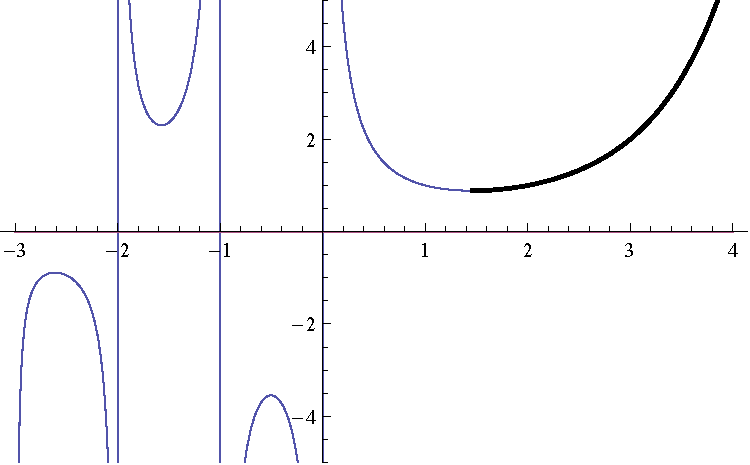
\includegraphics[width=4in]{images/plot-gamma-bold.pdf} 
\caption{Plot of $\Gamma(x)$ ({\bf invertible}, {\color{blue} real}, {\color{red} imaginary})}
\label{fig:gamma}
\end{center}
\end{figure}

The gamma function is the unique solution to:
\begin{equation}
\left\{\begin{array}{ll}
\Gamma(1) = 1 & \ \\
\Gamma(z+1) = z \Gamma(z) & \forall z \in \CC \\
\frac{d^2}{dz^2} \log \Gamma(z) \ge 0 & \forall z > 0
\end{array}\right\}
\end{equation}

The gamma function is very well known, but mostly as the analytic continuation of the factorial, meaning it extends the following product to complex $n$:
\begin{equation}
n! = \prod_{k=1}^{n} k = \Gamma(n+1)
\end{equation}


\subsection{Barnes $G$ function (super-factorial)}
\begin{defn}
The {\bf Barnes $G$ function} is 
\begin{equation}\notag
G(z+1) := \sqrt{(2\pi)^{z}/\exp\left(z+z^2(1 + \gamma)\right)}
\prod_{n=1}^{\infty}\left[\left(1+\frac{z}{n}\right)^n\exp\left(\frac{z^2}{2n} - z\right)\right]
\end{equation}
\end{defn}

\begin{figure}[h]
\begin{center}
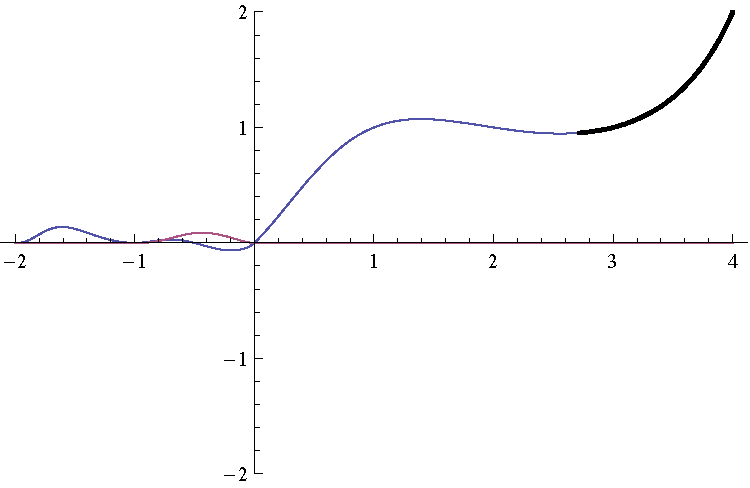
\includegraphics[width=4in]{images/plot-barnesg-bold.pdf} 
\caption{Plot of $G(x)$ ({\bf invertible}, {\color{blue} real}, {\color{red} imaginary})}
\label{fig:barnesg}
\end{center}
\end{figure}

Another definition is $G(z+1) = \exp\left( z \log \Gamma(z) + \zeta'(-1)-\zeta'(-1, z) \right)$ where $\zeta(t, z)$ is the Hurwitz zeta function, and $\zeta'(t, z) = \frac{d}{dt}(t, z)$.

The Barnes $G$ function is the unique solution to:
\begin{equation}
\left\{\begin{array}{ll}
G(1) = 1 & \ \\
G(z+1) = \Gamma(z)G(z) & \forall z \in \CC \\
\frac{d^3}{dz^3} \log G(z) \ge 0 & \forall z > 0
\end{array}\right\}
\end{equation}

The Barnes $G$ function extends the following product to complex $n$:
\begin{equation}
n\$ = \prod_{k=1}^{n} k! = G(n+2)
\end{equation}
where $n\$$ is the super-factorial.
\subsubsection{References for the Barnes $G$ function}
\begin{enumerate}
\item V. S. Adamchik, {\it Contributions to the Theory of the Barnes Function}, \\
{\small $<$http://www-2.cs.cmu.edu/{\textasciitilde}adamchik/articles/barnes1.pdf$>$}.
\item V. S. Adamchik, {\it Symbolic and Numeric Computation of the Barnes Function},
{\small $<$http://math.unm.edu/ACA/2001/Proceedings/SymNum/Adamchik\_paper.pdf$>$}.
\item E. W. Barnes, {\it The Theory of the Double Gamma Function}, Philosophical Transactions of the Royal Society of London. ser. A, {\bf 196} (1901): 265-387.
\item E. W. Barnes, {\it The Theory of the $G$-function}, Quarterly Journal of Pure and Applied Mathematics {\bf 31} (1900): 265-314.
\item Ashkan Nikeghbali; Marc Yor, {\it The Barnes $G$ function and its relations with sums and products of generalized Gamma convolution variables}, arXiv, \\
{\small $<$http://arxiv.org/abs/0707.3187v1$>$}.
\item Eric W. Weisstein, {\it Barnes $G$-function}, MathWorld, \\
{\small $<$http://mathworld.wolfram.com/BarnesG-Function.html$>$}.
\item {\it Barnes $G$-function}, {\small $<$http://en.wikipedia.org/wiki/Barnes\_G-function$>$}.
\end{enumerate}

\subsection{Fox $\mu$ function (change of base formula)}

TODO

\subsection{Galidakis $HW$ function (hyper-product-logarithm)}
\begin{defn}
The {\bf Galidakis $HW$ function} is
\begin{equation}
HW_{k}(c_1, \cdots, c_n; \ z) = w \text{ where } w \towerhuge{k=1}{n} (\ee^{c_k}; w) = z
\end{equation}
\end{defn}
According to Galidakis, a Taylor series expansion of an $HW$ function is:
\begin{equation}\notag
HW(\mathbf{c}; w) = z_0 + \sum_{n=1}^{\infty}\frac{(w-w_0)^n}{n!}
\left\{\frac{d^{n-1}}{dz^{n-1}}\left[\frac{z-z_0}{G(z)-w_0}\right]^n
\right\}_{z=z_0}
\end{equation}
where
\begin{equation}\notag
G(z) = z \towerhuge{n=1}{m} (\ee^{c_n}; z)
\end{equation}
which he derives using the Lagrange Inversion Theorem.

\begin{figure}[p]
\begin{center}
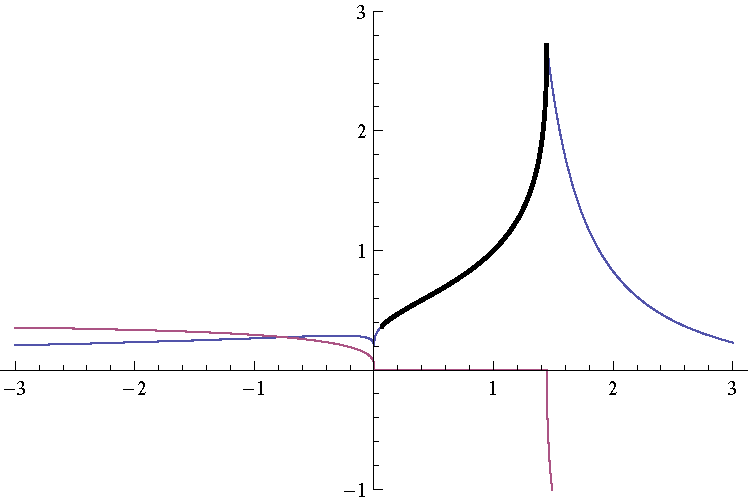
\includegraphics[width=4in]{images/plot-tetrate-bold.pdf} 
\caption{Plot of $H(x) = {}^{\infty}x$ ({\bf converge}, {\color{blue} real}, {\color{red} imaginary})}
\label{fig:inftetrate}
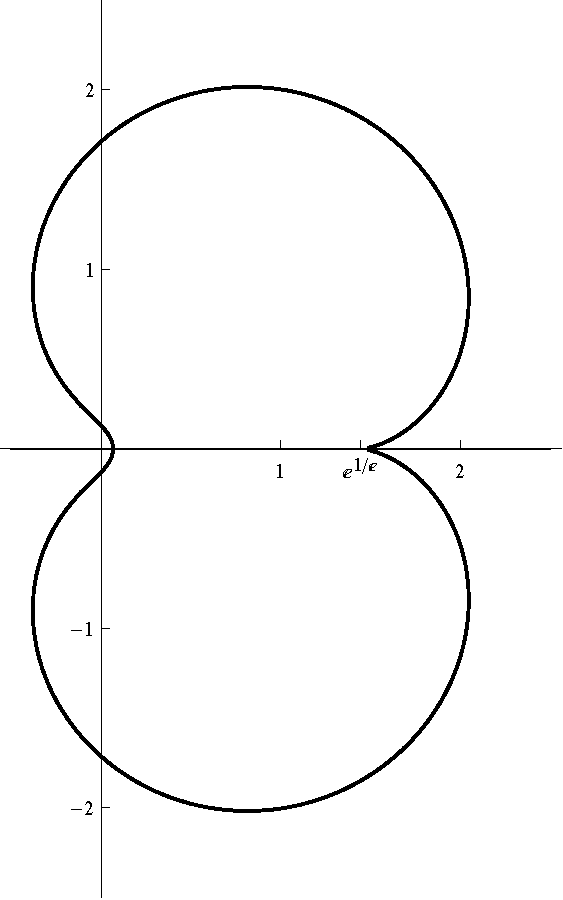
\includegraphics[height=3in]{images/region-shell-line.pdf} 
\quad\quad\quad\quad
 {\raise 0.4in \hbox{
\includegraphics[height=2in]{images/region-shell.png}}} 
\caption{Region of convergence of $\displaystyle \lim_{n\rightarrow\infty} {}^{n}x$}
\label{fig:region}
\end{center}
\end{figure}

\subsection{Knoebel $H$ function (infinitely iterated exponential)}
%20070809 Trappmann's 7 "Infinite Power Towers"
\begin{defn}
The {\bf infinitely iterated exponential} is $H_L(x) = \displaystyle \lim_{n\rightarrow\infty}{}^{n}x$.
\end{defn}
\begin{defn}
The {\bf Knoebel $H$ function} is $H_k(x) = \exp\left(-{W_{(-k)}(-\log(x))}\right)$
\end{defn}

Another version of this function by Galidakis is $h_k(x) = \exp\left(-{W_{k}(-\log(x))}\right)$ but this gives the wrong branch structure, because $h_0(x) < h_{(-1)}(x)$ whereas with the definition above $H_0(x) < H_{1}(x)$ which coincides with the real branch structure. We can use $H$ and $h$ to distinguish between the two branch structures of this function.

In Knoebel's 1981 paper \cite{Knoebel1981}, he asked three questions: ``{\it When does  $x^y < y^x$}'', ``{\it When does  $x^y = y^x$}'' and ``{\it Is there a formula for $y = f(x)$}''. For the first question, see the section on {iterated exponentials}. For the second and third question, see the section on the {exponential commutator}. The exponential commutator can be found through the different branches of the Knoebel $H$ function,  described here.

The infinitely iterated exponential $(H_{L})$ is the first form of tetration, and its convergence is the first theorem of tetration. In 1783, Euler proved that $H_L$ converges on the positive real axis if and only if $\ee^{-\ee} \le x \le \ee^{1/\ee}$, later discussed by Eisenstein in 1844. Since both Euler and Eisenstein were the first to talk about $H_L$, this interval is sometimes known as the {\bf Euler-Eisenstein interval}.

The infinitely iterated exponential spawned research into nested exponentials, 
where Barrow \cite{Barrow} and others sought converges tests comparable to those available for infinite series. Although few convergence tests exist, Bachman \cite{Bachman} concludes that with the addition of his proof of the {\bf Ramanujan convergence test}, 
the theory of the convergence of infinitely nested exponentials is complete.

The theory of infinitely iterated exponentials had been worked on by Shell in his thesis \cite{Shell}. Thron \cite{Thron} had come close to a complete parameterization of the region in the complex plane where $H_L$ converges, but left some points out. Shell proved that $H_L(\ee^{\zeta \ee^{-\zeta}})$ converges to $\ee^\zeta$ if $|\zeta| < 1$. This region is illustrated in figure (\ref{fig:region}), and is sometimes called the {\bf Shell-Thron region}. Shell then went on to derive a convergence test for infinitely iterated exponentials with arbitrary top exponent, where he shows that $\exp_{(\ee^{\zeta \ee^{-\zeta}})}^\infty(z)$ converges to $\ee^\zeta$ if and only if $|\zeta| < 1$ and:
\begin{equation}
\boxed{
|z - \ee^\zeta| < r |\ee^\zeta|
}
\end{equation}
where $r$ is a positive root of the equation $\log(1+r)/r = |\zeta|$.

A general derivative of the Knoebel $H$ function is:
\begin{equation}
H'(x) = \frac{H(x)^2}{x(1-H(x)\log(x))}
\end{equation}
which can be turned into a differential equation by cross multiplying, which in turn can be solved by the Frobenius method to obtain the coefficients. Fortunately, the coefficients have already been found, and there are two well-known expansions for this function, one due to Eissenstein \cite{Eissenstein}, and the other due to Jovovic.

A Puiseux series expansion of $H$ is:
\begin{thm}%checked
\begin{equation}
{}^{\infty}{x} = \sum^{\infty}_{k=0} \frac{\log(x)^k}{k!}  (k+1)^{(k-1)}
\end{equation}
\end{thm}
A Taylor series expansion of $H$ is:
\begin{thm}[Jovovic {[A033917]}]%checked
\begin{equation}
{}^{\infty}{x} = \sum^{\infty}_{k=0} \frac{(x - 1)^k}{k!} \sum^k_{j=0} \stirfirst{k}{j} (j+1)^{(j-1)}
\end{equation}
\end{thm}



\subsection{Lambert $W$ function (product-logarithm)}

\begin{figure}[h]
\begin{center}
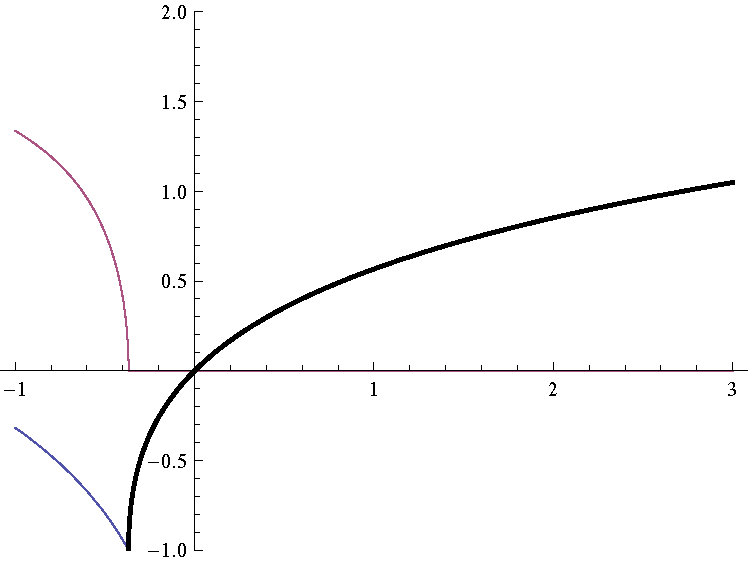
\includegraphics[width=4in]{images/plot-prodlog-bold.pdf} 
\caption{Plot of $W(x)$ ({\bf invertible}, {\color{blue} real}, {\color{red} imaginary})}
\label{fig:prodlog}
\end{center}
\end{figure}

\begin{defn}
The {\bf Lambert $W$ function} is defined by $W(x)\ee^{W(x)} = x$.
\end{defn}

The Lambert $W$ function is the most important function in its class, because it is available in most major computer algebra systems (CAS) as a built-in function. It is available in Maple as \verb"LambertW("$x$\verb")" and in Mathematica as \verb"LambertW["$x$\verb"]".

A closely related function is defined as $T(x) = -W(-x)$, which is known as the tree function.

A general derivative of the Lambert $W$ function is:
\begin{equation}
W'(x) = \frac{W(x)}{x(1+W(x))}
\end{equation}

\subsection{Munafo class function}
In Munafo's website about {\it Large Numbers} \cite{MunafoLN}
he describes a number class system. His description is based on the {\it perception class} of a real number, possibly large. The {\bf Munafo class} system starts by defining class-0 numbers as 1 through 6. Munafo then gives an upper-bound for class-1 at about $10^6$, and for class-2 numbers at about $10^{10^6}$. This is obviously a super-logarithmic scale, so we can use the super-logarithm to simplify his description. 

Let the Munafo class of $n$ be denoted $MC(n)$. The class function satisfies:
\begin{equation}
\exp^{MC(n) - 1}_{10}(6) < n \le \exp^{MC(n)}_{10}(6)
\end{equation}
Replace 6 with $\exp^{\slog_{10}(6)}_{10}(1)$, and add hyper-exponents:
\begin{align}
\exp^{MC(n) - 1}_{10}{\left(\exp^{\slog_{10}(6)}_{10}(1)\right)}
& < n \le \exp^{MC(n)}_{10}{\left(\exp^{\slog_{10}(6)}_{10}(1)\right)} \\
\exp^{MC(n) - 1 + \slog_{10}(6)}_{10}(1) 
& < n \le \exp^{MC(n) + \slog_{10}(6)}_{10}(1)
\end{align}
Take the super-log of each side, then subtract $MC(n) + \slog_{10}(6)$ from each side:
\begin{align}
MC(n) - 1 + \slog_{10}(6) < \slog_{10}(n) \le MC(n) &{} + \slog_{10}(6) \\
- 1 < \slog_{10}(n) -  \slog_{10}(6) - MC(n) &{} \le 0 \\
\lceil \slog_{10}(n) -  \slog_{10}(6) - MC(n) &{} \rceil = 0
\end{align}

Since the middle is always between $-1$ and 0 (but never $-1$), the ceiling of the middle is always zero.
Using (7.6), we can take $MC(n)$ outside the ceiling, because it is an integer, so we can summarize the Munafo class $MC(n)$ of a number $n$ as:
\begin{equation}
MC(n) = \lceil \slog_{10}(n) - \slog_{10}(6) \rceil
\end{equation}

%{Other Number Classes}
%{Ackermann Numbers}
%\begin{equation}
%A_n = n \uparrow^{n} n
%\end{equation}
%{Mersene Numbers}
%\begin{equation}
%M_n = 2^n - 1
%\end{equation}

\subsubsection{Munafo class of named large numbers}
\begin{center}
\begin{tabular}{c|l|r|l}
$MC(n)$ & $\slog_{10}(n)$ & $n$ & Name \\
\hline
\hline
$-1$ & $-1$ & $0$ & zero \\
\hline
$0$ & $0$ & $1$ & one \\
$0$ & $0.39312$ & $2$ & two \\
$0$ & $0.58836$ & $3$ & three \\
$0$ & $0.70801$ & $4$ & four \\
$0$ & $0.79068$ & $5$ & five \\
$0$ & $0.85223$ & $6$ & six \\
\hline
$1$ & $0.90044$ & $7$ & seven \\
$1$ & $0.93957$ & $8$ & eight \\
$1$ & $0.97220$ & $9$ & nine \\
$1$ & $1$ & $10$ & ten \\
$1$ & $1.39312 $ & $100$ & hundred \\
$1$ & $1.58836 $ & $1000$ & thousand \\
$1$ & $1.85223 $ & $10^6$ & million \\
\hline
$2$ & $1.97220 $ & $10^9$ & billion \\
$2$ & $2.01411$ & ${}^{\pi}{\boldsymbol{e}} \approx 3.7149 \times 10^{10}$ & e-tetra-pi \\
$2$ & $2.31648$ & $|M| \approx 8.0801 \times 10^{53}$ & monster group order \\
$2$ & $2.36588$ & $136 \times 2^{256} \approx 1.5748 \times 10^{79}$ & Eddington's number \\
$2$ & $2.39312$ & $10^{100}$ & googol \\
\hline
$3$ & $3.39312$ & $10^{10^{100}}$ & googol-plex \\
\end{tabular}
\end{center}

%{Unclassified Numbers}
%\begin{description}
%\item[mega] $=  M(2,1,5)$
%\item[megiston] $=  M(10,1,5)$
%\item[Moser's number] $=  M(2,1,M(2,1,5))$
%\item[Graham's number] $=  g^{64}(4)$ where $g(n) = 3 \uparrow^{n} 3$
%\item[3rd Ackermann number] $=  A_3 = 3 {\uparrow}{\uparrow}{\uparrow} 3 = {}^{7625597484987}3$
%\end{description}

%########## Chapter: Special Functions
%########## Section: Special cases of exponentials

\section{Special cases of exponentials}
\subsection{Decremented exponentials}
\subsection{Product exponentials}
Product exponentials $PE_b(z) = z b^z$ are not very common, except in certain partial differential equations. When they arise, they usually arise with base $\ee$, so the form $PE(z) = PE_{\ee}(z)$ is the most common.

\begin{figure}[h]
\begin{center}
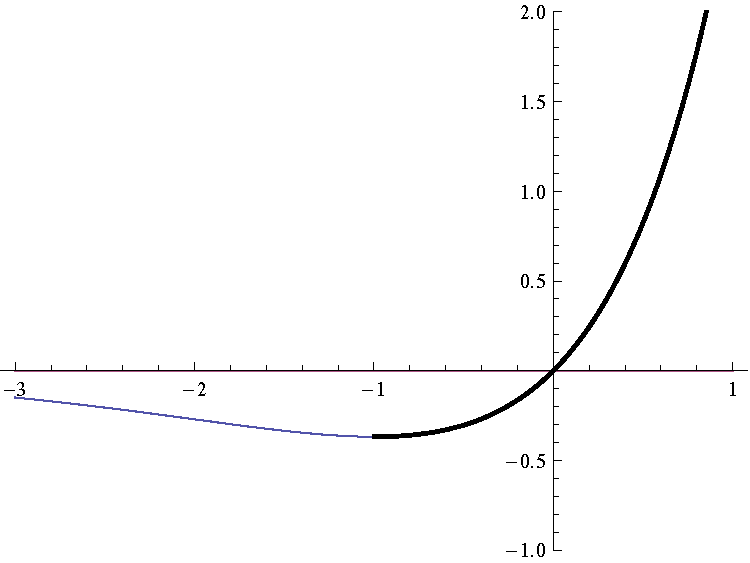
\includegraphics[width=4in]{images/plot-prodexp-bold.pdf} 
\caption{Plot of $x \ee^x$ ({\bf invertible}, {\color{blue} real}, {\color{red} imaginary})}
\label{fig:prodexp}
\end{center}
\end{figure}



\subsection{Scaled exponentials}
Work on the dynamics of the "exponential map" rarely talk about $\exp_x(z) = x^z$. Daniel Geisler [?] has done some initial research into the dynamics of $\exp_x$. However, Devaney [?] and others have written extensive investigations into the map $SE_\lambda (z) = \lambda \ee^z$. The dynamics of $SE_\lambda$ do not immediately imply the same properties of $\exp_x$, but we can relate them by noticing that: 
\begin{align}
SE_\lambda(\lambda z) & = \lambda{\ee}^{\lambda z} = \lambda \exp_{(\ee^\lambda)}(z) \\
SE^{\circ 2}_\lambda(\lambda z) & = \lambda{\ee}^{\lambda{\ee}^{\lambda z}} = \lambda \exp^{\circ 2}_{(\ee^\lambda)}(z) \\
SE^{\circ 3}_\lambda(\lambda z) & = \lambda{\ee}^{\lambda{\ee}^{\lambda{\ee}^{\lambda z}}} = \lambda \exp^{\circ 3}_{(\ee^\lambda)}(z)
\end{align}
and since this pattern obviously continues indefinitely, we find the relationship:
\begin{equation}
\boxed{
SE^{\circ n}_\lambda(\lambda z) = \lambda \exp^{\circ n}_{(\ee^\lambda)}(z)}
\end{equation}
for all integer $n$, which allows theorems about one to be converted into the other.

%########## Chapter: Special Functions
%########## Section: Special cases of tetration

\section{Special cases of tetration}
\subsection{Half-exponential}
\begin{defn}
The {\bf half-exponential} is $\exp^{\circ 1/2}_b(x)$.
\end{defn}

TODO

\subsection{Self-power}
\begin{defn}
The {\bf self-power} is $SP(x) := x^x = {}^{2}x$.
\end{defn}

\begin{figure}[h]
\begin{center}
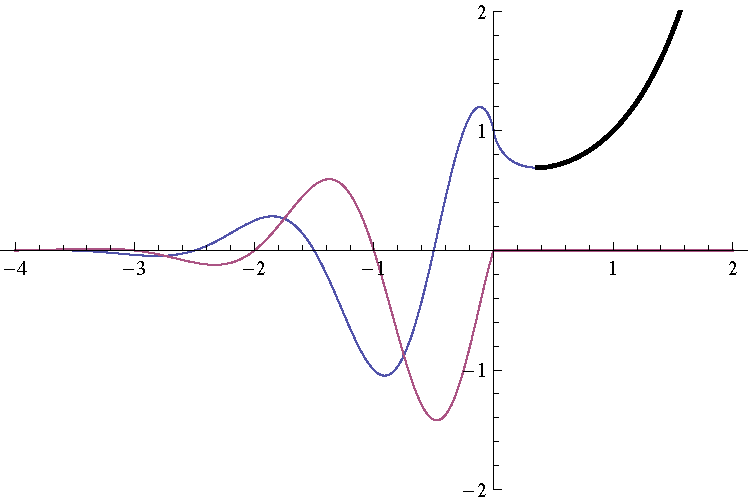
\includegraphics[width=4in]{images/plot-selfpow-bold.pdf} 
\caption{Plot of $x^x$ ({\bf invertible}, {\color{blue} real}, {\color{red} imaginary})}
\label{fig:selfpower}
\end{center}
\end{figure}

Although this is a simple case of tetration, it is non-trivial since the immediate answer most would give for a power series expansion of ${{}^{2}}{x} = x^x$ is the exponential expansion $x^x = \ee^{x \log(x)} = \sum_k \frac{x^k \log(x)^k}{k!}$ which is not a Taylor series in $x$. Below are the Puiseux and Taylor series in $x$ for this special case. They can be found through differentiation of $x^x$ or $\ee^{x{\ee}^{x}}$, and the closed-forms for the exponential coefficients can be found in Sloane's OEIS [?].
[how its related to polygon notation]

A Puiseux series expansion:
\begin{thm}%checked
\begin{equation}
{{}^{2}}{x} = \sum^{\infty}_{k=0} \frac{\log(x)^k}{k!} \sum^k_{j=1} \binom{k}{j} j^{(k-j)}
\end{equation}
\end{thm}
A Taylor series expansion:
\begin{thm}[Jovovic {[A005727]}]%checked
\begin{equation}
{}^{2}{x} = \sum^{\infty}_{k=0} \frac{(x-1)^k}{k!} \sum^{k}_{j=0} \stirfirst{k}{j} \sum^j_{i=0} \binom{j}{i} i^{(j-i)}
\end{equation}
where $0^0=1$.
\end{thm}

{Iterated Second Hyperpowers}
We begin with the integer iterates:
\begin{align}
SP^{\circ 1}(x) = {x^x} & = \tower{}(x, x, 1) \\
SP^{\circ 2}(x) = {{(x^x)}^{(x^x)}} & = \tower{}(x, x, 1 + x) \\
SP^{\circ 3}(x) = {{{(x^x)}^{(x^x)(x^x)^{(x^x)}}}} & = \tower{}(x, x, 1 + x + x^{1+x})
\end{align}
this leads us to notice that the third tower element is a sum of terms that satisfy the recurrence equation:
$c_{n+1}(x) = c_n(x) + x^{c_n(x)}$ where $c_1(x) = 1$.
which allows the iterate family of Frappier exponentials to be written:
$FE^{[n]}(x) = \tower{}\left(x, x, c_n(x)\right)$,
however, this affords very little insight into the flow of Frappier exponentials.

two methods that work:
* Lagrange interpolation of iterate-derivative matrix about $x=1$ (only works because parabolic)
* non-integer matrix powers of Bell matrix of $SH(x+1)-1$

\begin{align}
SP^{\circ t}(x)
& = 1 + (x-1) + t (x-1)^2 \notag \\
& + \left(-\frac{1}{2}t + t^2 \right)(x-1)^3 \notag\\
& + \left(\frac{7}{12}t - \frac{5}{4}t^2 + t^3 \right)(x-1)^4 \\
& + \left(-\frac{7}{8}t + \frac{17}{8}t^2 - \frac{13}{6}t^3 + t^4 \right)(x-1)^5 \notag \\
& + \left(\frac{169}{120}t - \frac{49}{12}t^2 + \frac{119}{24}t^3 - \frac{77}{24}t^4 + t^5 \right)(x-1)^6 + \cdots \notag
\end{align}

\subsection{Self-root}
\begin{defn}
The {\bf self-root} is $x^{1/x}$.
\end{defn}

\begin{figure}[h]
\begin{center}
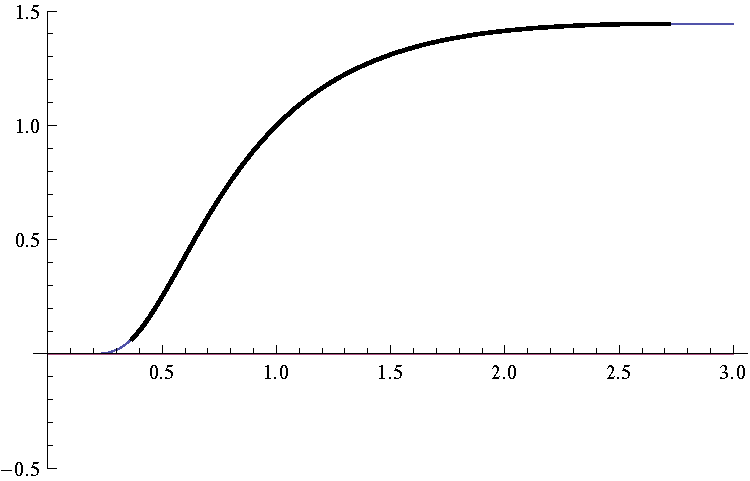
\includegraphics[width=4in]{images/plot-selfroot-bold.pdf} 
\caption{Plot of $x^{1/x}$ ({\bf converge}, {\color{blue} real}, {\color{red} imaginary})}
\label{fig:selfroot}
\end{center}
\end{figure}

\begin{thm}[Jovovic {[A008405]}]%checked
\begin{equation}
x^{1/x} = \sum^{\infty}_{k=0} \frac{(x-1)^k}{k!} \sum^{k}_{j=0} \stirfirst{k}{j} \sum^{j}_{i=0} \binom{j}{i} (-i)^{(j-i)}
\end{equation}
\end{thm}

\begin{thm}[Jovovic {[A003725]}]%checked
\begin{equation}
x^{1/x} = \sum^{\infty}_{k=0} \frac{\log(x)^k}{k!} \sum^{k}_{j=0} \binom{k}{j} (-j)^{(k-j)}
\end{equation}
\end{thm}

\begin{thm}[{[A081048]}]
\begin{equation}
\log(x^{1/x}) = \sum^{\infty}_{k=0} {(x - 1)^k} (-1)^{k+1} \sum^k_{j=1} \frac{1}{j}
\end{equation}
\end{thm}


\subsection{Super-sqrt (ssqrt)}
\begin{defn}
The {\bf super-sqrt} is $\ssqrt_k(x) = \exp\left({W_{k}(\log(x))}\right)$.
\end{defn}
\begin{figure}[h]
\begin{center}
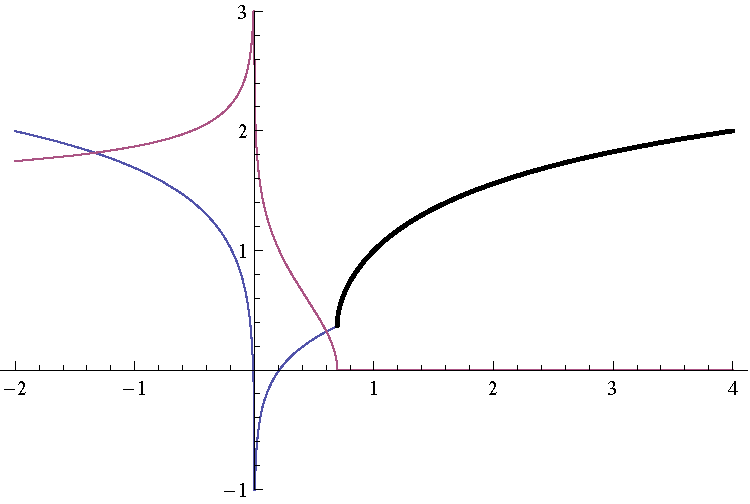
\includegraphics[width=4in]{images/plot-ssqrtx-bold.pdf} 
\caption{Plot of $\ssqrt(x)$ ({\bf invertible}, {\color{blue} real}, {\color{red} imaginary})}
\label{fig:supersqrt}
\end{center}
\end{figure}

\begin{thm}[Jovovic {[A120980]}]%checked
\begin{equation}
\boxhyperroot{4}{2}{x} = \sum^{\infty}_{k=0} \frac{(x-1)^k}{k!} \sum^{k}_{j=0} \stirfirst{k}{j} (1-j)^{(j-1)}
\end{equation}
\end{thm}
\begin{thm}[not double-checked]
\begin{equation}
\log(\boxhyperroot{4}{2}{x}) = \sum^{\infty}_{k=0} \frac{(x-1)^k}{k!} \left( \frac{(-1)^k}{k+1} \right) \sum^{k+1}_{j=1} \left| s^{(k+1)}_j \right| j^{(j-1)}
\end{equation}
\end{thm}

A general derivative of $\ssqrt(x)$ is:
\begin{equation}
\ssqrt'(x) = \frac{\ssqrt(x)}{x(\log(x) + \ssqrt(x))}
\end{equation}

The second super-root $\boxhyperroot{4}{2}{z} = x$ solves the equation $x^x = z$ for $x$.
An obvious alternative to using a function to solve this example equation is by using iteration. Before we can use iteration we must take the $x$-th root of both sides to get $x = z^{1/x}$ and take the reciprocal of both sides to get $1/x = (1/z)^{1/x}$. By replacing $1/x$ with $(1/z)^{1/x}$ repeatedly, we obtain an infinitely iterated exponential $1/x = {}^{\infty}(1/z)$. Now that there is only one $x$ in the expression we can take the reciprocal again to find the relationship between the second super-root and infinitely iterated exponentials:
\begin{equation}\label{superroot2}
\boxhyperroot{4}{2}{z} = x = \frac{1}{{}^{\infty}(1/z)}
\end{equation}

A similar relationship can be found with the Lambert $W$-function. Starting with the definition of the second super-root we have already obtained $x = z^{1/x}$, and dividing by $x$ gives $1 = (1/x)z^{1/x}$ so we can manipulate the equation into the form $w \ee^w = z$ used by the definition of the Lambert $W$-function. Substitute $z = \ee^{\log(z)}$ to get $1 = (1/x)\ee^{\log(z)/x}$, and multiply by $\log(z)$ to get 
$\log(z) = (\log(z)/x) \ee^{\log(z)/x}$, and since the equation is of the form of the definition of the Lambert $W$-function, we have $W(\log(z)) = \log(z)/x$. This involves only one $x$ so solving gives the relationship between the second super-root and the Lambert $W$-function:
\begin{equation}
\boxhyperroot{4}{2}{z} = x = \frac{\log(z)}{W(\log(z))}
\end{equation}

At this point one could note that these techniques will only work for the second super-root, and not the third or fourth, because iteration would be so much more complicated in these and other cases. There is, however, one other super-root that can be simplified like the second super-root can; the infinite super-root. The infinite super-root is defined as $\srt_{\infty}(z) = x$ if and only if ${}^{\infty}x = z$ but we already know that the inverse function is $x = z^{1/z} = \sqrt[z]{z}$ by definition. Interestingly, this can be manipulated into a form that looks very similar to (\ref{superroot2}), by taking the reciprocal of the reciprocal an equivalent expression is obtained:
\begin{equation}
\srt_{\infty}(z) = x = \sqrt[z]{z} = \frac{1}{{}^{2}(1/z)}
\end{equation}
Our aim is to understand the many relationships that exist between infinitely iterated exponentials, the second super-root, and the Lambert $W$-function, one of which shows that the first two are {\it strangely commutative} with respect to 2 and $\infty$:
\begin{equation}\notag
\boxed{
\begin{array}{c}
\srt_{2}(z) ={1}/{{}^{\infty}{({1}/{z})}} \\
\srt_{\infty}(z) ={1}/{{}^{2}{({1}/{z})}}
\end{array}
}
\end{equation}

For more information see the section on topological conjugacy.

%########## Chapter: Special Functions
%########## Section: Miscellaneous functions

\section{Miscellaneous functions}

\subsection{Exponential commutator}
\begin{defn}
The {\bf exponential commutator} is defined as:
\begin{equation}
EC(x) = y \text{ where } x^y = y^x \text{ and } x \ne y
\end{equation}
The exponential commutator is one of the functions Knoebel [?] discusses in his review of iterated exponentials.
\end{defn}
This can be found for $x \in \RR$ by:
\begin{equation}
EC(x) = \begin{cases}
H_{1}({x}^{1/x})& \text{if }x < \ee, \\
H({x}^{1/x}) & \text{if }x > \ee.
\end{cases}
\end{equation}
it is debatable whether or not $EC(\ee) = \ee$ since this would not satisfy (1).

\begin{question}
When does $x^y = y^x$?
\end{question}


\subsection{Exponential factorial}
\begin{defn}
The {\bf exponential factorial} is ${E\!F}(x) = x^{{E\!F}(x-1)}$ where $E\!F(1) = 1$.
\end{defn}

Other initial conditions such as $E\!F(0) = 0$ have also been used before [?].

The exponential factorial may be written in tower notation as:
\begin{equation}
E\!F(x) = \towerhuge{k=0}{\infty} (x - k)
\end{equation}

Using this it is interesting to approximate the extension of the exponential factorial to the real numbers using this, where the tower is "chopped off" at some point, for example:
\begin{equation}
E\!F(x) \approx \towerhuge{k=0}{10} (x - k)
\end{equation}
or
\begin{equation}
E\!F(x) \approx \begin{cases}
\log_{x+1}(E\!F(x+1)) & \text{if } x < 1\\
f(x) & \text{if } 1 \le x \le 2 \\
x^{E\!F(x-1)} & \text{if } x > 2 
\end{cases}
\end{equation}
where $f(x)$ is an approximation such as:
\begin{align}
f(x) \approx 1 &+ 0.575571 (x-1) + 0.229718 (x-1)^2 + 0.0785761(x-1)^3 \\
f(x) \approx 1 &+ 0.570807 (x-1) + 0.232292 (x-1)^2 \\
&+ 0.114153 (x-1)^3 + 0.0234736 (x-1)^4\notag
\end{align}

Using these approximations, or any for that matter, the 3-cycle that dominates the infinite tetration fractal\footnote{see here}, is somewhat apparent in various graphs of $EF$.

%########## Chapter: Special Functions
%########## Section: Topological Conjugacy

\section{Topological Conjugacy}

\subsection{Exponential-like conjugates}
Exponential-like conjugates satisfy the following diagram:
\begin{diagram} 
\log_b(z) & & & \rTo{b^x = (h^{1/h})^x} & & & (z) \\
 & \luTo^{h(x+1)} & & & & \ruTo^{h(x+1)} & \\
\dTo^{\lambda x} & & \CC & \rTo^{h^x-1} & \CC & & \dTo_{\lambda x} \\
 & \ldTo^{\lambda h (x+1)} & & & & \rdTo^{\lambda h (x+1)} & \\
\CC & & & \rTo^{\lambda \ee^x = \log(b) \ee^x} & & & \CC
\end{diagram}
where $b = \ee^{\lambda} = h^{1/h}$ and $h = H(b) = {}^{\infty}b$ and $\lambda = \log(b)$.

\subsection{Lambert-like conjugates}
Lambert-like conjugates satisfy the following diagram:
\begin{diagram} 
\CC & & & \rTo^{x^x} & & & \CC \\ 
 & \luTo^{\ee^x} & & & & \ruTo^{\ee^x} & \\
\dTo^{\frac{1}{x}} & & W(z) & \rTo^{x\ee^x} & (z) & & \dTo_{\frac{1}{x}} \\
 & \ldTo^{\ee^{-x}} & & & & \rdTo^{\ee^{-x}} & \\
\CC & & & \rTo{x^{1/x}} & & & \CC
\end{diagram}





\appendix

\chapter{Function symbols}
\begin{tabular}{l|l}
Symbol & Function Name \\
\hline
$AS$ & Helm's alternating tetration series \\
$B\!A$ & Bowers' array notation \\
$C\!A$ & Conway's chained arrow notation \\
$C\!N$ & Nelson's hyper-logarithm transform \\
$D\!E$ & decremented exponentials $(\ee^x - 1)$ \\
$EC$ & exponential commutator $(x^y = y^x)$ \\
$E\!F$ & exponential factorial \\
$EG$ & exponential gamma function \\
$H$ & Knoebel $H$ function, infinitely iterated exponential \\
$HC$ & critical piece of hyper-operations over real hyper-exponents \\
$H\!D$ & critical piece of hyper-operations over real ranks \\
$H\!E$ & half-exponential function \\
$H\!F$ & Frappier hyper-operations \\
$H\!R$ & Robbins hyper-operations \\
$HT$ & Trappmann hyper-operations \\
$HW$ & Galidakis $HW$ function, hyper-product-logarithms \\
$I\!G$ & Ioannis Galidakis' extension of tetration \\
$M\!C$ & Munafo class function \\
$P\!E$ & product exponentials $(x \ee^x)$ \\
$R\!M$ & Robert Munafo's extension of tetration \\
$S\!E$ & Devaney's scaled exponentials $(c \ee^x)$ \\
$S\!M$ & Steinhaus-Moser polygon notation \\
$S\!P$ & self-power function, second tetrate $(x^x)$\\
$S\!R$ & self-root function, infinite super-root $(x^{1/x})$\\
%$\srt$ & super-root \\
%$\slog$ & super-logarithm \\
$W$ & Lambert $W$ function, base-$e$ product-logarithm
\end{tabular}

\chapter{Tables of values}
In the table below, 
%{\bf bold} areas indicate where methods are approximately equal, 
(BC${}_2$) is used because of $3 \times 3$ matrix power rules in some CASs, (DG${}_3$) is used because Geisler gives terms 0-3 explicitly in [?], 
for (SW), $w$ has been chosen such that ${}^{(-1/2)}{\ee} = 1/2$, 
and average values are used for (CN${}^{-1}$).
\begin{center}\small
Table 2: ${}^{y}{\ee}$ for $y \in [-1,1]$. \\
\begin{tabular}{c||c|c|c|c|c|c||c|c}
$y$&Lin&BC${}_2$&DG${}_5$&IG&RM&SW&AR${}^{-1}_{10}$&CN${}^{-1}_{10}$\\
\hline
-1	& 0 & {\bf 0} & $0.241 + 0.326 \ii$ &  &  &  & 0 &  \\
-0.9	& 0.1 & {\bf 0.1}055 & $0.394 + 0.170 \ii$ &  &  &  & 0.1062 &  \\
-0.8	& 0.2 & {\bf 0.2}072 & $0.475 + 0.034 \ii$ &  &  &  & 0.2079 &  \\
-0.7	& 0.3 & {\bf 0.3}063 & $0.508 - 0.060 \ii$ &  &  &  & 0.3063 &  \\
-0.6	& 0.4 & {\bf 0.4}036 & $0.524 - 0.105 \ii$ &  &  &  & 0.4029 &  \\
-0.5	& 0.5 & {\bf 0.5}000 & $0.547 - 0.106 \ii$ &  &  &  & 0.4986 &  \\
-0.4	& 0.6 & {\bf 0.5}964 & ${\bf 0.5}93 - 0.081 \ii$ &  &  &  & 0.5946 &  \\
-0.3	& 0.7 & {\bf 0.6}937 & ${\bf 0.6}67 - 0.046 \ii$ &  &  &  & 0.6917 &  \\
-0.2	& 0.8 & {\bf 0.7}928 & ${\bf 0.7}66 - 0.018 \ii$ &  &  &  & 0.7910 &  \\
-0.1	& 0.9 & {\bf 0.8}945 & ${\bf 0.8}80 - 0.002 \ii$ &  &  &  & 0.8934 &  \\
0 	& 1 & 1 & 1 &  &  &  & 1 &  \\
0.1	& 1.1052 & {\bf 1.1}100 & ${\bf 1.1}19 - 0.007 \ii$ & 0.0000 & 0.0000 & 0.0000 & 1.1121 & 0.0000 \\
0.2	& 1.2214 & {\bf 1.2}258 & ${\bf 1.2}37 - 0.016 \ii$ &  &  &  & 1.2310 &  \\
0.3	& 1.3499 & {\bf 1.3}483 & ${\bf 1.3}56 - 0.022 \ii$ &  &  &  & 1.3584 &  \\
0.4	& 1.4918 & {\bf 1.4}786 & ${\bf 1.4}84 - 0.021 \ii$ &  &  &  & 1.4961 &  \\
0.5	& 1.6487 & {\bf 1.6}180 & ${\bf 1.6}26 - 0.015 \ii$ &  &  &  & 1.6465 &  \\
0.6	& 1.8221 & 1.7678 & ${\bf 1.7}89 - 0.006 \ii$ &  &  &  & 1.8123 &  \\
0.7	& 2.0138 & 1.9293 & ${\bf 1.9}77 + 0.003 \ii$ &  &  &  & 1.9971 &  \\
0.8	& 2.2255 & 2.1040 & ${\bf 2.1}91 + 0.008 \ii$ &  &  &  & 2.2055 &  \\
0.9	& 2.4596 & 2.2937 & ${\bf 2.4}32 + 0.010 \ii$ &  &  &  & 2.4433 &  \\
1	& $\ee$ & 2.5 & $2.702 + 0.017 \ii$ &  &  &  & $\ee$ & ?
\end{tabular}
\end{center}

\chapter{Series expansions}
{Exponential Coefficient Tables}
A listing follows of the first 10 (or so) exponential coefficients of tetration functions:

\begin{center}
Table 3: $A_{nk}$ where ${}^{n}{x} = \sum^{\infty}_{k=0} \frac{A_{nk} \log(x)^k}{k!}$
\begin{tabular}{c|ccccccccccc}
$n,k$&0&1&2&3&4&5&6&7&8&9&10\\
\hline
1	&1&1&1&1&1&1&1&1&1&1&1\\
2	&1&1&3&10&41&196&1057&6322&41393&293608&2237921\\
3	&1&1&3&16&101&756&6607&65794&733833&9046648&121961051\\
4	&1&1&3&16&125&1176&12847&160504&2261289&35464816&612419291\\
5	&1&1&3&16&125&1296&16087&229384&3687609&66025360&1303751051\\
6	&1&1&3&16&125&1296&16807&257104&4480569&87238720&1874561291\\
7	&1&1&3&16&125&1296&16807&262144&4742649&96915520&2197675691\\
8	&1&1&3&16&125&1296&16807&262144&4782969&99637120&2323474091\\
9	&1&1&3&16&125&1296&16807&262144&4782969&100000000&2354318891\\
\hline
${\infty}$&1&1&3&16&125&1296&16807&262144&4782969&100000000&2357947691
\end{tabular}
\end{center}

\begin{center}
Table 8: $A_{nk}$ where ${}^{n}(x; z) = \sum^{\infty}_{k=0} \frac{A_{nk} \log(x)^k}{k!}$
\begin{tabular}{c|cccccc}
$n,k$&0&1&2&3&4&5\\
\hline
1	&1&$z$&$z^2$&$z^3$&$z^4$&$z^5$\\
2	&1&1&$1+2z$&$1+6z+3z^2$&$1+12z+24z^2+4z^3$&$1+20z+90z^2+80z^3+5z^4$\\
3	&1&1&3&$10+6z$&$41+48z+12z^2$&$196+360z+180z^2+20z^3$\\
4	&1&1&3&16&$101+24z$&$756+360z+60z^2$\\
5	&1&1&3&16&125&$1176+120z$\\
6	&1&1&3&16&125&1296\\
\hline
${\infty}$&1&1&3&16&125&1296
\end{tabular}
\end{center}

\begin{center}
Table 4: $A_{nk}$ where ${}^{n}{x} = \sum^{\infty}_{k=0} \frac{A_{nk} (x - 1)^k}{k!}$
\begin{tabular}{c|ccccccccccc}
$n,k$&0&1&2&3&4&5&6&7&8&9&10\\
\hline
1	&1&1&0&0&0&0&0&0&0&0&0\\
2	&1&1&2&3&8&10&54&-42&944&-5112&47160\\
3	&1&1&2&9&32&180&954&6524&45016&360144&3023640\\
4	&1&1&2&9&56&360&2934&26054&269128&3010680&37616880\\
5	&1&1&2&9&56&480&4374&47894&574888&7829424&116392080\\
6	&1&1&2&9&56&480&5094&60494&823528&12365424&206078880\\
7	&1&1&2&9&56&480&5094&65534&944488&15359184&274118880\\
8	&1&1&2&9&56&480&5094&65534&984808&16629264&312523680\\
9	&1&1&2&9&56&480&5094&65534&984808&16992144&327038880\\
\hline
${\infty}$&1&1&2&9&56&480&5094&65534&984808&16992144&330667680
\end{tabular}
\end{center}

\begin{center}
Table 8: $A_{nk}$ where ${}^{n}(x; z) = \sum^{\infty}_{k=0} \frac{A_{nk} (x - 1)^k}{k!}$
\begin{tabular}{c|cccccc}
$n,k$&0&1&2&3&4&5\\
\hline
1	&1&$z$&$-z+z^2$&$2z-3z^2+z^3$&$-6z+11z^2-6z^3+z^4$&$24z-50z^2+35z^3-10z^4+z^5$\\
2	&1&1&$2z$&$3z^2$&$-2z+6z^2+4z^3$&$10z-45z^2+40z^3+5z^4$\\
3	&1&1&2&$3+6z$&$8+12z+12z^2$&$10+90z+60z^2+20z^3$\\
4	&1&1&2&9&$32+24z$&$180+120z+60z^2$\\
5	&1&1&2&9&56&$360+120z$\\
6	&1&1&2&9&56&480\\
\hline
${\infty}$&1&1&2&9&56&480
\end{tabular}
\end{center}

\begin{center}
Table 5: $A_{nk}$ where $\log({}^{n}{x}) = \sum^{\infty}_{k=0} \frac{A_{nk} (x - 1)^k}{(k+1)!}$
\begin{tabular}{c|ccccccccccc}
$n,k$&0&1&2&3&4&5&6&7&8&9\\
\hline
2	&1&1&-1&2&-6&24&-120&720&-5040&40320\\
3	&1&1&5&2&44&-96&986&-6056&52272&-466920\\
4	&1&1&5&26&104&804&4136&38296&247320&2586000\\
5	&1&1&5&26&224&1524&15896&149176&1830384&21682560\\
6	&1&1&5&26&224&2244&23456&297016&3947184&60263760\\
7	&1&1&5&26&224&2244&28496&377656&5852304&96551760\\
8	&1&1&5&26&224&2244&28496&417976&6759504&122255760\\
9	&1&1&5&26&224&2244&28496&417976&7122384&133142160\\
\hline
${\infty}$&1&1&5&26&224&2244&28496&417976&7122384&136770960
\end{tabular}
\end{center}
\ 
\newline

And a listing of the first 10 (or so) exponential coefficients of super-root functions:

\begin{center}
Table 6: $A_{nk}$ where $\srt_n(z) = \sum^{\infty}_{k=0} \frac{A_{nk} \log(z)^k}{k!}$
\begin{tabular}{c|ccccccccccc}
$n,k$&0&1&2&3&4&5&6&7&8&9&10\\
\hline
2	&1&1&-1&4&-27&256&-3125&46656&-823543&16777216&-387420489\\
3	&1&1&-1&-2&33&-184&-695&32124&-369215&-1298816&143686161\\
4	&1&1&-1&-2&9&116&-1175&-3786&92449&1565416&-41559759\\
5	&1&1&-1&-2&9&-4&625&-7146&-33551&821512&-2333439\\
6	&1&1&-1&-2&9&-4&-95&5454&-60431&-312488&8371521\\
7	&1&1&-1&-2&9&-4&-95&414&40369&-554408&-2968479\\
8	&1&1&-1&-2&9&-4&-95&414&49&352792&-5387679\\
9	&1&1&-1&-2&9&-4&-95&414&49&-10088&3684321\\
\hline
${\infty}$&1&1&-1&-2&9&-4&-95&414&49&-10088&55521
\end{tabular}
\end{center}

\begin{center}
Table 7: $A_{nk}$ where $\srt_n(z) = \sum^{\infty}_{k=0} \frac{A_{nk} (z-1)^k}{k!}$
\begin{tabular}{c|ccccccccccc}
$n,k$&0&1&2&3&4&5&6&7&8&9&10\\
\hline
2	&1&1&-2&9&-68&740&-10554&185906&-3891320&94259952&-2592071760\\
3	&1&1&-2&3&28&-510&4926&-10500&-900304&26247816&-392237520\\
4	&1&1&-2&3&4&30&-2094&33810&-338176&3412080&-93913560\\
5	&1&1&-2&3&4&-90&1506&-28350&444704&-5489064&47130840\\
6	&1&1&-2&3&4&-90&786&-630&-166816&4490136&-79146360\\
7	&1&1&-2&3&4&-90&786&-5670&75104&-2132424&55724040\\
8	&1&1&-2&3&4&-90&786&-5670&34784&226296&-22597560\\
9	&1&1&-2&3&4&-90&786&-5670&34784&-136584&2804040\\
\hline
${\infty}$&1&1&-2&3&4&-90&786&-5670&34784&-136584&-824760
\end{tabular}
\end{center}

\begin{center}
Table 8: $A_{nk}$ where $\log(\srt_n(x)) = \sum^{\infty}_{k=0} \frac{A_{nk} (x - 1)^k}{(k+1)!}$
\begin{tabular}{c|cccccccccc}
$n,k$&0&1&2&3&4&5&6&7&8&9\\
\hline
2	&1&-3&17&-146&1704&-25284&456224&-9702776&237711888&-6593032560\\
3	&1&-3&11&-26&-266&6336&-73662&166608&18635328&-604483080\\
4	&1&-3&11&-50&394&-5364&82788&-1262064&20814120&-426484080\\
5	&1&-3&11&-50&274&-1044&-14652&562416&-12551184&242958960\\
6	&1&-3&11&-50&274&-1764&18108&-351504&8193456&-184206240\\
7	&1&-3&11&-50&274&-1764&13068&-69264&-1332144&73136160\\
8	&1&-3&11&-50&274&-1764&13068&-109584&1389456&-36030240\\
9	&1&-3&11&-50&274&-1764&13068&-109584&1026576&-6999840\\
\hline
${\infty}$&1&-3&11&-50&274&-1764&13068&-109584&1026576&-10628640
\end{tabular}
\end{center}


\chapter{Credits}
%20070809 Trappmann's 8 "Coming in Contact"
\ 

TODO

% The desired format is based on AMS + MLA, for Journal articles I try to follow:
% <Author>;<Author2>, {\it <Title>}, <Journal> {\bf <Vol>}.<No> (<Year>): <Pages>.
% If anyone wants to use pure AMS or pure MLA please make sure all are consistent.
%These references should include as much information as possible, regardless of whether it follows AMS or MLA formats. As such, both Journal references and PDF references should be included, if possible. Some reference are incomplete, and are difficult to find more information about, due to extreme abbreviations, see \cite{Koch1900} for an example of this. The only abbreviations that should be used are very, very common ones like "Math." and "Sci." All others should be avoided.

% All references to www.mathsoft.com are talking about a page:
% http://www.mathsoft.com/mathsoft_resources/mathsoft_constants/ref/2118.asp
% which now gives a 404 error, but at one time listed 26 references, included here.

\begin{thebibliography}{100}
\bibitem{Abel1881}
	Niels Henrik Abel, {\it Oeuvres compl{\`e}tes},
	 Christiania (Oslo), Gr{\o}ndahl \& S{\o}n, {\bf 2}.6 (1881): 36-39.
	{-- Also referenced in \cite{Knoebel1981}}.
\bibitem{AbramowitzStegun}
	M. Abramowitz and I. A. Stegun, 
	{it Handbook of Mathematical Functions}, 
	Dover, 1972; %MR 94b:00012.
	% -- also ref'd by www.mathsoft.com which is no longer available.
\bibitem{Ackermann1928} 
	W. Ackermann, 
	{\it Zum Hilbertschen Aufbau der reel len Zahlen},
	Math. Annalen {\bf 99} (1928): 118�133. 
	{-- Also referenced in \cite{Knoebel1981}}.
% [AJR] can't find a way to make this fit on the page.
%\bibitem{AczelRoteSchwaiger} 
%	J. Acz{\'e}l; G. Rote; J. Schwaiger, 
%	{\it Webs, Iteration Groups and Equivalent Changes in Probabilities}. 
%	Quarterly of Applied Mathematics 54 (1996), 475-499
%	{\small $<$http://www.inf.fu-berlin.de/{\textasciitilde}rote/Papers/pdf/Webs,+iteration+groups,+and+equivalent+changes+in+probabilities.pdf$>$}.
%	{-- Also referenced in \cite{KindermannRefs}}.
\bibitem{AlsedaKolyadaLlibreSnoha}
	Ll. Alsed{\'a}, S. Kolyada, J. Llibre; L. Snoha, 
	{\it Axiomatic definition of the topological entropy on the interval}. 
	Preprint CRM \#458, Centre de Recerca Matematica, Barcelona. 
	To appear in Aequationes Math.(2000)
	{\small $<$http://www.imath.kiev.ua/{\textasciitilde}skolyada/Axent0.pdf$>$}.
	{-- Also referenced in \cite{KindermannRefs}}.
\bibitem{Allen1969}
	Arnold O. Allen, 
	{\it $\ee^\pi$ or $\pi^\ee$?} 
	J. Recreational Math. {\bf 2} (1969): 255-256.
	{-- Also referenced in \cite{Knoebel1981}}.
\bibitem{AndrewsLacher1977}
	J. J. Andrews; R. C. Lacher, {\it Stacked exponents},
	Aequationes Math. {\bf 16} (1977): 137-147.
	{-- Also referenced in \cite{Knoebel1981}}.
\bibitem{Apostol1957}
	Tom M. Apostol,
	{\it Mathematical Analysis},
	Addison-Wesley, 1st ed.
	(1957): 383. Exercise 12-7.
	{-- Also referenced in \cite{Knoebel1981}}.
\bibitem{Ash1996}
	J. M. Ash, 
	{\it The limit of $x^{x^{\cdot^{\cdot^{x}}}}$ as $x$ tends to zero},
	Math. Mag. {\bf 69}.3 (1996), 207-209. 
\bibitem{Aldrovandi}
	R. Aldrovandi,
	{\it Special Matrices of Mathematical Physics} where??.
\bibitem{AldrovandiFreitas1998}
	R. Aldrovandi and L.P. Freitas,
	{\it Continuous Iteration of Dynamical Maps},
	Journal of Math. Phys. {\bf 39} (1998): 5324-5336.
	{-- Also referenced in \cite{KindermannRefs}}.
\bibitem{Bachman1995}
	G. Bachman,
	{\it Convergence of Infinite Exponentials},
	Pacific Journal of Math. {\bf 169}, 2, 1995.
\bibitem{BakerMaalouf1995}
	I. N. Baker and R. N. Maalouf, 
	{\it Convergence of a modified iteration process}, 
	Computational Methods and Function Theory, Proc. 1994 Penang conf., 
	World Sci. Publishing, (1995); MR 97k:30030.
	% -- also ref'd by www.mathsoft.com which is no longer available.
\bibitem{BakerRippon1985}
	I. N. Baker; P. J. Rippon, 
	{\it A note on complex iteration},
	American Math. Monthly, {\bf 92}.7 (1985): 501-504. 
	%MR801229 (86m:30024)
	%; MR 86m:30024.
	% -- also ref'd by www.mathsoft.com which is no longer available.
\bibitem{BakerRippon1989}
	I. N. Baker; P. J. Rippon, 
	{\it Towers of exponentials and other composite maps}, 
	Complex Variables Theory Appl. {\bf 12} (1989): 181-200. %; MR 91b:30068.
	% -- also ref'd by www.mathsoft.com which is no longer available.
\bibitem{Barrow}
	D. F. Barrow, 
	{\it Infinite Exponentials},
	American Math. Monthly {\bf 43}.3 (Mar. 1936): 150-160.
	% -- also ref'd by www.mathsoft.com which is no longer available.
\bibitem{Bell1938}
	E. T. Bell, 
	{\it The Iterated Exponential Integers},
	The Annals of Mathematics, 2nd Ser., {\bf 39}.3 (Jul. 1938): 539-557. 
\bibitem{Bierens}
	B. C. Berndt, 
	Ramanujan's Notebooks: Part IV, Springer-Verlag, (1994): 308.
	%; MR 95e:11028.
	% -- also ref'd by www.mathsoft.com which is no longer available.
\bibitem{Bierens}
	D. Bierens de Haan, 
	{\it Nouvelles tables d'integrales definies}, 
	Hafner, 1957 (1867 ed., corrected); table 278, formula 17.
	% -- also ref'd by www.mathsoft.com which is no longer available.
\bibitem{BorweinCorless1999}
	J. M. Borwein and R. M. Corless, 
	{\it Emerging tools for experimental mathematics}, 
	American Math. Monthly 106 (1999) 889-909.
	% -- also ref'd by www.mathsoft.com which is no longer available.
\bibitem{BowersAN} 
	Jonathan Bowers, 
	{\small $<$http://members.cox.net/hedrondude/array.htm$>$}
\bibitem{BriggsW}
	K. Briggs, W-ology or some exactly solvable growth models (University of Cambridge).
	% -- also ref'd by www.mathsoft.com which is no longer available.
\bibitem{Bromer1987}
	Nick Bromer, 
	{\it Superexponentiation}, 
	Mathematics Magazine, {\bf 60}.3 (1987): 169-174.
\bibitem{Brunson1986}
	B. W. Brunson, 
	{\it The partial order of iterated exponentials},
	American Math. Monthly {\bf 93} (1986): 779-786
	%; MR 89d:06001.
	% -- also ref'd by www.mathsoft.com which is no longer available.
\bibitem{Carleman}
	Torsten Carleman,
	{\it Application de la th{\'e}orie des {\'e}quations int{\'e}grales lin{\'e}aires 
	aux syst{\`e}mes d'{\'e}quations diff{\'e}rentielles non lin{\'e}aires}.
	Acta Mathematica {\bf 59} (1932).
	%DOI: 10.1007/BF02546499.
\bibitem{Carmichael}
	R. D. Carmichael,
	{\it On certain transcendental functions},
	American Math. Monthly, {\bf 15} (1908): 78.
	{-- Also referenced in \cite{MacDonnell}}.
\bibitem{Clenshaw1986}
	C. W. Clenshaw; D. W. Lozier; F. W. J. Oliver; P. R. Turner, 
	{\it Generalized exponential and logarithmic functions},
	Comput. Math. Appl., {\bf 12B} (5/6) (1986): 1091-1101.
\bibitem{Clenshaw1989}
	C. W. Clenshaw; F. W. J. Oliver; P. R. Turner, 
	{\it Level-index arithmetic: an introductory survey},
	Numerical Analysis and Parallel Processing (P. R. Turner, ed.), 
	Lecture Notes in Math., Springer-Verlag, New York, {\bf 1397} (1989).
\bibitem{CohenVillegasZagier}
	H. Cohen, F. Rodriguez Villegas and D. Zagier, 
	{\it Convergence acceleration of alternating series}, 
	Experim. Math. 9 (2000) 3-12; preprint.
	% -- also ref'd by www.mathsoft.com which is no longer available.
\bibitem{Comtet1974}
	L. Comtet,
	{\it Advanced Combinatorics}, Reidel, Dordrecht, (1974).
	{-- Also referenced in \cite{KindermannRefs}}.
\bibitem{CorlessJeffreyKnuthOLW}
	R.M. Corless, G. H. Gonnet, D. E. G. Hare, D.J. Jeffrey, and D.E. Knuth,
	{\it On the Lambert W function},
	Adv. Comput. Math. {\bf 5} (1996): 329-359.
	%preprint; MR 98j:33015.
	% -- also ref'd by www.mathsoft.com which is no longer available.
\bibitem{CorlessJeffreyKnuthSSLW}
	R.M. Corless, D.J. Jeffrey, and D.E. Knuth,
	{\it A Sequence of Series for the Lambert W-function},
	Proceedings of the 1997 International Symposium on Symbolic and Algebreic 
	Computation, Maui, Hawaii. New York: ACM Press, 197-204, 1997.
\bibitem{CreutzSternheimerFQ}
	M. Creutz; R. M. Sternheimer, 
	{\it On the convergence of iterated exponentiation}, 
	Fibonacci Quarterly, 
	18 (1980) 341-347; 
	19 (1981) 326-335; 
	20 (1982) 7-12; 
	%MR 82b:26006, MR 83b:26006 and MR 83i:26002.
	% -- also ref'd by www.mathsoft.com which is no longer available.
\bibitem{Cunningham1916}
	Alan Cunningham,
	{\it Factorisation of $N = (x^y + y^x)$}.
	Messenger of Math. {\bf 45} (1916): 185-192.
	{-- Also referenced in \cite{Knoebel1981}}.
\bibitem{Dainelli1889}
	Ugo Dainelli,
	{\it Sull'equazione $x^y = y^x$ con $x$ ed $y$ interi e positivi}.
	Periodico di Matematica {\bf 4} (1889): 115-117.
	{-- Also referenced in \cite{Knoebel1981}}.
\bibitem{Dawson1994}
	R. J. MacG. Dawson, 
	{\it Towers of Powers Modulo $m$},
	The College Math. Journal, {\bf 25}.1 (1994): 22-28.
\bibitem{DevaneyKrych1984}
	R. L. Devaney; M. Krych, 
	{\it Dynamics of $\exp(z)$},
	Ergodic Theory Dynamical Systems, 
	{\bf 4} (1984): 35-52.
\bibitem{Dickson1919}
	Leonard E. Dickson,
	{\it A History of the Theory of Numbers},
	Carnegie Institution of Washington {\bf 2} (1919): 687.
\bibitem{Eisenstein1844}
	G. Eisenstein,
	{\it Entwicklung von $a^{a^{\cdot^{\cdot}}}$},
	Crelle's Journal f\"ur die reine und 
	Angewandte Math. {\bf 28} (1844):  49-52.
	{-- Also referenced in \cite{Knoebel1981}}.
\bibitem{ErdosJabotinskyOAI}
	P. Erd{\"o}s; E. Jabotinsky, 
	{\it On Analytic Iteration}. 
	Journal Analyse Math. 8 (1960/61), 361-376.
	{-- Also referenced in \cite{KindermannRefs}}.
\bibitem{Euler1748}
	L. Euler,
	{\it Introductio in analysin infinitorum}, (1748) 
	Reprinted by Culture et Civilization, Brussels {\bf 2} (1967): 293-295.
	{-- Also referenced in \cite{Knoebel1981}}.
\bibitem{Euler1778}
	L. Euler, 
	{\it De formulis exponentialibus replicatis},
	Acta Academiae Scientarum Imperialis Petropolitinae {\bf 1} (1778), 38�60. 
	Reprinted in Opera Omnia, Series Prima {\bf 6} (?): 268-297.
	{-- Also referenced in \cite{Knoebel1981}}.
\bibitem{Euler1783}
	L. Euler, 
	{\it De serie Lambertina Plurimisque eius insignibus proprietatibus},
	Acta Acad. Scient. Petropol. 2, 29-51, 1783. 
	%Reprinted in Euler, L. Opera Omnia, Series Prima, Vol. 6: 
	%Commentationes Algebraicae. pp. 350-369. 
\bibitem{Fatou1919}
	P. Fatou, 
	{\it Sur les {\'e}quations fonctionelles},
	Bull. Soc. Math. France, 
	{\bf 47} (1919): 161-271; 
	{\bf 48} (1920): 33-94 and 208-314.
	{-- Also referenced in \cite{Walker1991}}.
\bibitem{Flechsenhaar}
	A. Flechsenhaar, 
	{\it Ueber die Gleichung $x^y = y^x$}.
	Unterrichtsbl{\"a}tter f{\"u}r Math. {\bf 17} (1911): 70-73.
	{-- Also referenced in \cite{Knoebel1981}}.
\bibitem{Franklin1917}
	Philip Franklin,
	{\it Relating to the real locus defined by the equation $x^y = y^x$}.
	American Math. Monthly {\bf 24} (1917): 137.
	{-- Also referenced in \cite{Knoebel1981}}.
\bibitem{GeislerTO}
	Daniel Geisler, 
	{\it What lies beyond exponentiation?}, {\small $<$http://www.tetration.org/$>$}.
\bibitem{GoebelNederpelt}
	F. G{\"o}bel; R. P. Nederpelt,
	{\it The number of numerical outcomes of iterated powers},
	American Math. Monthly {\bf 78} (1971): 1097-1103.
	{-- Also referenced in \cite{Knoebel1981}, \cite{MacDonnell}}.
\bibitem{GoodsteinP1957}
	Peter Goodstein,
	{\it The iterated exponential of $x$}.
	Math. Gazette {\bf 41} (1957): 219.
	{-- Also referenced in \cite{Knoebel1981}}.
\bibitem{GoodsteinP1958}
	Peter Goodstein,
	{\it Limits of iterated logarithmic functions}
	Math. Gazette {\bf 42} (1958): 295-296.	
	{-- Also referenced in \cite{Knoebel1981}}.
\bibitem{Goodstein1947}
	R. L. Goodstein, 
	{\it Transfinite Ordinals in Recursive Number Theory}, 
	Journal of Symbolic Logic, {\bf 12}.4 (1947).
	Note: this is the first appearance of the term {\it tetration}.
\bibitem{Goodstein1958}
	R. L. Goodstein,
	{\it The system of equations $b^{x_n} = x_{n+1}$},
	Math. Gazette {\bf 42} (1958): 296-299. 
	{-- Also referenced in \cite{Knoebel1981}}.
\bibitem{GalidakisCEH4}
	I. N. Galidakis, 
	{\it A continuous extension for the hyper4 operator},
	Available: {\small $<$http://users.forthnet.gr/ath/jgal/math/exponents4.html$>$}
\bibitem{GalidakisEH4}
	I.N. Galidakis,
	{\it On Extending hyper4 and Knuth's Up-arrow Notation to the Reals}, where?.
\bibitem{GalidakisHW}
	I. N. Galidakis, 
	{\it On solving the $p$-th complex auxiliary equation $f^{(p)}(z) = z$},
	Complex Variables, {\bf 50}.13 (Oct. 2005): 977-997.
\bibitem{GalidakisHWD}
	I. N. Galidakis, 
	{\it General Properties of and Differential Equations Solvable by the HW Functions},
	Available: {\small $<$...$>$}.
\bibitem{GalidakisHWFunc}
	I. N. Galidakis, 
	{\it On Some Applications of the Generalized Hyper-Lambert Functions},
	Available: {\small $<$...$>$}.
\bibitem{GralewiczKowalski}
	P. Gralewicz and K. Kowalski,
	{\it Continuous time evolution from iterated maps and Carleman linearization}, where?.
%\bibitem{Gosper}
%	R. W. Gosper, e-message (September 1997).
%	% -- also ref'd by www.mathsoft.com which is no longer available.
\bibitem{Grzegorczyk}
	Andrzej Grzegorczyk,
	{\it Some classes of recursive functions},
	Instytut Matematyczny Polskiej Akademii Nauk, Warszawa (1953): 1-44.
	Also in Rozprawy Matematycne IV?
\bibitem{Hausner1961}
	Alvin Hausner,
	{\it Algebraic number fields and the Diophantine equation $m^n = n^m$}.
	American Math. Monthly {\bf 68} (1961): 856-861.
	{-- Also referenced in \cite{Knoebel1981}}.
\bibitem{Hengel}
	J. van Hengel,
	{\it Beweis des Satzes, das unter allen reellen positiven ganzen Zahlen nur das
	Zahlenpaar 4 und 2 f{\"u}r $a$ und $b$ der Gleichung $a^b = b^a$ gun{\"u}gt}.
	Progr. Emmerich, (1888).
	{-- Also referenced in \cite{Knoebel1981}, \cite{Dickson1919}}.
	Note: this is the first appearance of $x^y = y^x$.
	Hessel,
	{\it Ueber das merkw{\"u}rdige Beispiel einer zum Theil punctirt gebildeten Curve,
	das der Gleichung entspricht: $y = \sqrt[x]{x}$}.
	Archiv der Mathematik und Physik {\bf 14} (1850): 169-187.
\bibitem{Hurwitz1967}
	Solomon Hurwitz,
	{\it On the rational solutions of $m^n = n^m$ with $n \ne m$}.
	American Math. Monthly, {\bf 74} (1967): 298.
	{-- Also referenced in \cite{MacDonnell}}.
\bibitem{Iga}
	K. Iga, 
	{\it Continuous half-iterates of functions}. 
	{\small $<$http://math.pepperdine.edu/{\textasciitilde}kiga$>$}.
	{-- Also referenced in \cite{KindermannRefs}}.
\bibitem{Jabotinsky1963}
	E. Jabotinsky, 
	{\it Analytic iteration}. 
	Trans. Amer. Math. Soc. 108 (1963), 457-477
	{-- Also referenced in \cite{KindermannRefs}}.
\bibitem{Khovanskii1963}
	A. N. Khovanskii,
	{\it The Application of Continued Fractions and their 
	Generalizations to Problems in Approximation Theory}, 
	Noordhoff N. V., (1963); %MR 27 #6058.
	% -- also ref'd by www.mathsoft.com which is no longer available.
\bibitem{KindermannRefs}
	Lars Kindermann,
	{\it Iterative Roots and Fractional Iteration},
	Available: {\small $<$http://reglos.de/lars/ffx.html$>$}.
\bibitem{KlamkinGroeneveldOlds}
	M. S. Klamkin, R. A. Groeneveld and C. D. Olds, 
	{\it A comparison of integrals}, 
	American Math. Monthly 77 (1970) 1114 and 78 (1971) 675-676.
	% -- also ref'd by www.mathsoft.com which is no longer available.
\bibitem{Kneser1948}
	H. Kneser, 
	{\it Reelle analytische L{\"o}sungen der Gleichung 
	$\phi(\phi(x)) = \ee^x$ und verwandter Funktionalgleichungen},
	J. Reine Angew. Math. {\bf 187} (1948/50): 56-67.
	{-- Also referenced in \cite{KindermannRefs},\cite{Walker1991}}.
\bibitem{Knoebel1981}
	R. A. Knoebel, 
	{\it Exponentials reiterated},
	American Math. Monthly, {\bf 88}.4 (1981): 235-252.
	{-- Also referenced in \cite{MacDonnell}}.
	% -- also ref'd by www.mathsoft.com which is no longer available.
\bibitem{Koch1900}
	H. v. Koch, 
	Bil. t. Sv. Vet. Ak. Hand. 1, Math. 25, m\'em. no. 5, (1900): 1-24.
\bibitem{LaidlerLandau1977}
	P. Laidler; B. V. Landau,
	{\it A power sequence exercise for a pocket calculator}.
	Math. Gazette, {\bf 61} (1977): 191.
	{-- Also referenced in \cite{MacDonnell}}.
\bibitem{LopezOrtizFAQ}
	Alex L{\'o}pez-Ortiz
	Name for $f(x)^{f(x)} = x$, sci.math FAQ (Univ. of Waterloo).
	{\small $<$http://www.cs.uwaterloo.ca/{\textasciitilde}alopez-o/math-faq/math-faq.html$>$}.
	% -- also ref'd by www.mathsoft.com which is no longer available.
\bibitem{MacDonnell}
	J. MacDonnell, 
	{\it Some critical points of the hyperpower function $x^{x^{\cdot^{\cdot}}}$}, 
	International Journal of Math. Education {\bf 20}.2 (1989): 297-305.
	Available: \\
	{\small $<$http://www.faculty.fairfield.edu/jmac/ther/tower.htm$>$}.
	%MR994348 (90d:26003)
\bibitem{Macintyre1966}
	A. J. Macintyre, 
	{\it Convergence of $i^{i^{\cdot^{\cdot}}}$}, 
	Proc. American Math. Soc. 17 (1966) 67%; MR 32 #5855.
	% -- also ref'd by www.mathsoft.com which is no longer available.
\bibitem{Mauerer1901}
	H. Mauerer, 
	{\it \"Uber die Funktion $x^{x^{\cdot^{\cdot}}}$ f\"ur ganzzahliges Argument (Abundanzen)},
	Mitt. Math. Gesell. Hamburg 4, 33-50, 1901. \
\bibitem{Mitchelmore}
	M. C. Mitchelmore,
	{\it A matter of definition},
	American Math. Monthly, {\bf 81} (1974): 643.
	{-- Also referenced in \cite{MacDonnell}}.
\bibitem{MorrisSzekeres}
	K. W. Morris; G. Szekeres, 
	{\it Tables of the logarithm of iteration of $\ee^x - 1$},
	J. Austral. Math. Soc., {\bf 2} (1961-1962): 321-333.
\bibitem{MorrisSzekeres}
	E. J. Moulton,
	{\it The real function defined by $y^x = x^y$}.
	American Math. Monthly, {\bf 23} (1916): 233.
	{-- Also referenced in \cite{MacDonnell}}.
\bibitem{MuellerRA}
	Markus M{\"u}ller, {\it Reihenalgebra}, \\
	{\small $<$http://www.math.tu-berlin.de/{\textasciitilde}mueller/reihenalgebra.pdf$>$}
\bibitem{MunafoH4}
	Robert Munafo, 
	{\it Extension of the hyper4 function to the reals}, Available: \\
	{\small $<$http://home.earthlink.net/{\textasciitilde}mrob/pub/math/ln-notes1.html\#real-hyper4$>$}.
\bibitem{MunafoLN}
	Robert Munafo, 
	{\it Large Numbers}, \\
	{\small $<$http://home.earthlink.net/{\textasciitilde}mrob/pub/math/largenum.html$>$}.
\bibitem{NelsonMA}
	C. J. Nelson, {\it Progression of operations?}, \\
	{\small $<$http://www.math.niu.edu/{\textasciitilde}rusin/known-math/99/iteratedexp$>$}.
%\bibitem{Plouffe}
%	S. Plouffe, MRB constant (Plouffe's Inverter).
%	% -- also ref'd by www.mathsoft.com which is no longer available.
\bibitem{Pogorzelski1961}
	H. A. Pogorzelski, 
	{\it Problem 4976},
	The American Math. Monthly, {\bf 68}.6 (1961): 576-577.
%\bibitem{Pollack}
%	P. Pollack, USENET newsgroup (1998).
%	% -- also ref'd by www.mathsoft.com which is no longer available.
%\bibitem{PutnamA4}
%	Putnam Competition Problem A-4, American Math. Monthly 77 (1970) 723, 725.
%	% -- also ref'd by www.mathsoft.com which is no longer available.
\bibitem{Robbins2005}
	Andrew Robbins,
	{\it Solving for the analytic piecewise extension of tetration and the super-logarithm},
	Available: {\small $<$http://tetration.itgo.com/paper.html$>$}.
\bibitem{RubstovRomerio2003}
	C. A. Rubstov and G. F. Romerio, \\
	{\it Ackermann's Function and New Arithmetical Operation}, \\
	{\small $<$http://forum.wolframscience.com/showthread.php?threadid=956$>$}.
	{\small $<$http://forum.wolframscience.com/showthread.php?threadid=??$>$}.
	% http://www.rotarysaluzzo.it/filePDF/Iperoperazioni\%20(1).pdf
\bibitem{Rucker1995}
	R. Rucker,
	{\it Infinity and the Mind: The Science and Philosophy of the Infinite},
	Princeton, NJ: Princeton University Press, 1995.
\bibitem{ShellThesis}
	D. L. Shell,
	PHD Thesis.
\bibitem{Shell1962}
	D. L. Shell,
	{\it On the convergence of infinite exponentials},
	Proceedings of the American Math. Society {\bf 13} (1962): 678-681.
	% -- also ref'd by www.mathsoft.com which is no longer available.
\bibitem{Sloane7Seq2006}
	N. J. A. Sloane, 
	{\it Seven Staggering Sequences}, Available: 
	{\small $<$http://...$>$}.
\bibitem{Spiegel1968}
	M. R. Spiegel, 
	{\it Mathematical Handbook of Formulas and Tables}, 
	McGraw-Hill, (1968).
%\bibitem{Stewart2005}
%	J. Stewart,
%	{\it Single Variable Calculus: Concepts and Contexts},
%	Thomson Learning, 2005. \\
\bibitem{Sykora}
	Stanislav Sykora, 
	{\it Binary Iterated Powers}, Available: \\
	{\small $<$http://ebyte.it/library/docs/math06a/BinaryIteratedPowers.html$>$}.
\bibitem{Targonski1995}
	G. Targonski, 
	{\it Progress of iteration theory since 1981}. 
	Aequationes Math. 50 (1995), 50-72
	{-- Also referenced in \cite{KindermannRefs}}.
\bibitem{Thron1957}
	W. J. Thron, 
	{\it Convergence of infinite exponentials with complex elements},
	Proceedings of the American Mathematical Society, {\bf 8}.6 (Dec. 1957): 1040-1043.
	%; MR 20 #2552.
	% -- also ref'd by www.mathsoft.com which is no longer available.
\bibitem{TrappmannArbNum2006}
	H. Trappmann,
	{\it Arborescent Numbers: Higher Arithmetic Operations and Division Trees},
	{\small $<$http://math.eretrandre.org/tree-aoc/pdf/latest.pdf$>$}, (2006).
	% http://blafoo.de/tree-aoc/main1176.pdf
\bibitem{TrappmannSciMath2006}
	H. Trappmann; Ingolf Dahl,
	{\it Tetration extended to real exponents}, \\
	{\small $<$http://mathforum.org/kb/message.jspa?messageID=5434919\&tstart=0$>$}, (2006).
\bibitem{VilliersRobinson}
	J. M. de Villiers; P. N. Robinson,
	{\it The interval of convergence and limiting functions of a hyperpower sequence}, 
	American Math. Monthly {\bf 93} (1986): 13-23; 
	%MR 87d:26005. -- what is this MR stuff?
	% -- also ref'd by www.mathsoft.com which is no longer available.
\bibitem{Walker1991}
	Peter Walker, 
	{\it Infinitely Differentiable Generalized Logarithmic and Exponential Functions},
	Mathematics of Computation, {\bf 57}.196 (Oct. 1991): 723-733.
	{-- Also referenced in \cite{KindermannRefs}}.
\bibitem{Walker1988}
	Peter Walker, 
	{\it A class of functional equations which have entire solutions},
	Bull. Austral. Math. Soc., {\bf 39} (1988): 351-356.
	{-- Also referenced in \cite{Walker1991}}.
\bibitem{WalkerJM1991}
	Peter Walker, 
	{\it On the solutions of an Abelian functional equation},
	J. Math. Anal. Appl., {\bf 155} (1991): 93-110.
	{-- Also referenced in \cite{Walker1991}}.
\bibitem{Walker1990}
	Peter Walker, 
	{\it The exponential of iteration of $\ee^x - 1$},
	Proc. Amer. Math. Soc., {\bf 110} (1990): 611-620.
	{-- Also referenced in \cite{KindermannRefs}, \cite{Walker1991}}.
\bibitem{WeissteinCRC2002}
	Eric W. Weisstein, 
	{\it CRC Concise Encyclopedia of Mathematics}, Chapman \& Hall, (2002).
\bibitem{Wilf1990}
	Herbert S. Wilf, 
	{\it Generatingfunctionology}, Academic Press, (1990).
\bibitem{WolframNKS}
	Stephen Wolfram,
	{\it A New Kind of Science},
	Wolfram media.
\bibitem{WolframNKSOP}
	Stephen Wolfram,
	{\it A New Kind of Science: open problems and projects}, \\
	Available: {\small $<$http://www.wolframscience.com/openproblems/NKSOpenProblems.pdf$>$}
	[cited 13 July 2004].
\bibitem{WoonACO}
	S. C. Woon,
	{\it Analytic Continuation of Operators -- Operators acting complex $s$-times},
	{\small ?}, (accessed: 2006).
\bibitem{YukalovGluzman1999}
	Yukalov ..., where?.
\bibitem[A...]{SloaneA}
	N. J. A. Sloane,
	{\it Online Encyclopedia of Integer Sequences}, \\
	{\small $<$http://www.research.att.com/{\textasciitilde}njas/sequences/A...$>$}, (accessed: 2006).
%\bibitem{Tetraspace}
%	et. al.,
%	{\it Tetration and other large number sequences},
%	{\small http://tetraspace.alkaline.org/forum/viewtopic.php?t=248}
\end{thebibliography}

\end{document}
